\documentclass[inscr,ack,preface]{dithesis}

\usepackage{booktabs}
\usepackage{hyperref}
\usepackage{lipsum}
\usepackage{enumerate}
\usepackage{amsmath}
\usepackage{amssymb}
\usepackage{float}
\hypersetup{
    unicode=true,                     % non-Latin characters in bookmarks
    pdffitwindow=true,                % page fit to window when opened
    pdfnewwindow=true,                % links in new window
    pdfkeywords={},                   % list of keywords
    colorlinks=true,                  % false: boxed links; true: colored links
    linkcolor=black,                  % color of internal links
    citecolor=black,                  % color of links to bibliography
    filecolor=black,                  % color of file links
    urlcolor=black,                   % color of external links
    pdftitle={},                      % title
    pdfauthor={},                     % author
    pdfsubject={}                     % subject of the document
}


\authorFirstGr{Αλέξανδρος}
\authorFirstAbrGr{Α.} % abbreviation of first name
\authorMiddleGr{ΣΤΑ.}   % abbreviation of father's first name
\authorLastGr{Σταυρινουδάκης}
\authorFirstEn{Alexandros}
\authorFirstAbrEn{A.}
\authorMiddleEn{STA.}
\authorLastEn{Stavrinoudakis}
\authorSn{1115202200171}

\titleEn{The Design and Development of a Scene Editor in Virtual Reality}
\titleGr{Σχεδίαση και Ανάπτυξη Επεξεργαστή Σκηνών σε Περιβάλλον Εικονικής Πραγματικότητας}

\dateGr{ΜΑΪΟΣ 2026}
\dateEn{MAY 2026}

\supervisorGr{Μαρία Ρούσσου}{Αναπληρώτρια Καθηγήτρια}
\supervisorGr{Χρήστος Λουγιάκης}{Υποψήφιος Διδάκτωρ}
\supervisorEn{Maria Roussou}{Associate Professor}
\supervisorEn{Christos Lougiakis}{PhD Candidate}

\abstractEn{
This thesis explores the design and development of a Virtual Reality Scene Editor. 
Traditional three-dimensional environment design typically relies on two-dimensional displays, creating a 
cognitive gap between the creation process and the final immersive experience. By shifting the development 
workflow into a virtual reality environment, users can manipulate three-dimensional scenes with spatial awareness 
and scale accuracy that flat-screen editors cannot provide.

The developed application allows users to compose three-dimensional worlds using a library of predefined assets 
through intuitive spatial interactions. To assess the system's performance and usability, user experiments were 
conducted focusing on task efficiency and user presence.
}
\abstractGr{
Η πτυχιακή εργασία εξετάζει τη σχεδίαση και ανάπτυξη ενός επεξεργαστή σκηνών σε περιβάλλον Εικονικής Πραγματικότητας. 
Η παραδοσιακή σχεδίαση τρισδιάστατων περιβαλλόντων βασίζεται συνήθως σε
δισδιάστατες οθόνες, γεγονός που δημιουργεί ένα νοητικό κενό μεταξύ της διαδικασίας δημιουργίας και της τελικής εμπειρίας. 
Μεταφέροντας την επεξεργασία σκηνών σε περιβάλλον VR, οι χρήστες μπορούν να χειρίζονται τρισδιάστατες σκηνές με χωρική αντίληψη 
και ακρίβεια που οι επεξεργαστές επίπεδης οθόνης αδυνατούν να προσφέρουν.

Η εφαρμογή που αναπτύχθηκε επιτρέπει στους χρήστες να συνθέτουν τρισδιάστατους κόσμους χρησιμοποιώντας μια βιβλιοθήκη 
προκαθορισμένων αντικειμένων μέσω διαισθητικών χωρικών αλληλεπιδράσεων. Για την αξιολόγηση της απόδοσης 
και της χρηστικότητας του συστήματος, πραγματοποιήθηκαν πειράματα με χρήστες, εστιάζοντας στην αποτελεσματικότητα 
εκτέλεσης εργασιών και στην αίσθηση παρουσίας του χρήστη.
}
\acksEn{
I would like to thank my family and friends for their constant support and presence throughout these years.

I am incredibly grateful to my supervisor, Dr. Maria Roussou, for accepting to oversee this thesis and for her insightful guidance. 
Special thanks are also due to Dr. Christos Lougiakis for his dedicated support and valuable help at every stage of this project.

Lastly, I would like to thank all the participants of the experiments for their time and cooperation, without which this research 
would not have been possible.
}
\prefaceEn{
This thesis was developed as part of my undergraduate studies in the Department of Informatics and Telecommunications at the 
University of Athens.

I am deeply grateful to Dr. Maria Roussou and Dr. Christos Lougiakis for their continuous support and for sharing their expertise 
throughout this work.
}

\inscriptionEn{Dedicated to my family and my cat Tinker}

\subjectAreaGr{Αλληλεπίδραση Ανθρώπου Υπολογιστή}
\subjectAreaEn{Human-Computer Interaction}
\keywordsGr{Εικονική Πραγματικότητα, Επεξεργαστής Σκηνών}
\keywordsEn{Virtual Reality, Scene Editor}

%
% Set the .bib file containing your paper publications (leave the extension out)
%
% This is optional, but it should be specified when option 'lop' is passed to
% the document class.
%
% Then, inside the document environment, you may use the command '\nocitelop' to
% site your papers, as you would traditionally do with the commands '\cite' or
% '\nocite'.
%
% The papers are printed in reverse chronological order.
%
%\lopfile{mypapers/pubs}

\begin{document}

\frontmatter

\mainmatter

% add main chapters (should be given in capital letters)
\chapter{INTRODUCTION}

\section{Research Problem}
The creation of Virtual Reality (VR) content currently suffers from a fundamental ``paradigm mismatch.''
While the end product is an immersive 3D environment, the development process remains tethered to a 2D desktop workflow.
Traditional game engines utilize conventional WIMP (Windows, Icons, Menus, Pointers) interfaces that
were not designed for spatial computing.

This discrepancy forces developers into an inefficient, iterative loop:
\begin{enumerate}
  \item Modifying spatial properties (e.g., the height of a table) on a 2D monitor.
  \item Entering the VR environment to verify the ``sense of scale'' and ergonomic comfort.
  \item Exiting the VR environment to correct inaccuracies that were invisible in the 2D viewport.
\end{enumerate}

This constant ``context switching'' disrupts the creator's ``flow state'' and makes precise spatial design a matter
of trial and error rather than direct intuition.

\section{Motivation}

\subsection{The VR Content Gap}

The motivation for this thesis is driven by the widening ``content gap'' in the VR industry. Despite the rapid evolution of hardware
like the Meta Quest series, the complexity of the development pipeline remains a barrier to entry. By forcing creators to build 3D
worlds through a 2D lens, the industry limits the speed at which high-quality content can be produced.
Furthermore, as the industry moves toward ``Spatial Computing,'' there is a growing demand for tools that allow for \textit{in situ} creation.
Reducing the friction between the idea and the implementation is essential for both professional developers and the burgeoning
community of User-Generated Content (UGC) creators.

\subsection{NoFold}

NoFold is a next-generation web/XR hybrid platform developed by researchers at the National and Kapodistrian University of Athens,
designed to bridge the gap between digital board game development and the physical tabletop experience~\cite{Lougiakis2024NoFold}.
The platform aims to solve traditional playtesting challenges---such as high logistical costs, physical component constraints, and the
loss of social cues in standard digital platforms---by offering a two-part ecosystem: a web-based authoring hub for component creation and
asset management, and an immersive XR application (VR/MR) for realistic, physics-based playtesting and remote collaboration.

While the current iteration of NoFold successfully handles card game workflows and basic physics-based manipulation
(grabbing, moving, and throwing), to fully realize its potential as an all-in-one creation tool,
incorporating features for advanced environmental customization would be a highly useful addition to the platform's ecosystem.

\section{Purpose}
The objective of this research is the design and implementation of \textit{SceneEditorVR}, a functional VR-native scene editor prototype.
This project does not seek to replace comprehensive game engines but rather to investigate an immersive-first workflow for environmental
design and rapid prototyping.

The project focuses on the following core functionalities:
\begin{itemize}
  \item \textbf{Immersive Asset Management:} A VR-centric UI for navigating themed libraries and instantiating 3D models.
  \item \textbf{Natural Spatial Manipulation:} Leveraging 6DoF (Six Degrees of Freedom) input for intuitive translation, rotation,
        and scaling of objects.
  \item \textbf{Workflow Continuity:} Providing essential editor features—such as snapping, multi-selection, and undo/redo systems—entirely
        within the headset.
  \item \textbf{Data Portability:} Implementing a serialization system using readable .json and industry-standard .glb formats to ensure the
        VR-created scenes can be integrated back into traditional pipelines.
\end{itemize}

This thesis explores how moving the ``editor'' into the ``experience'' can streamline the creative process and democratize 3D
world-building.
\chapter{RESEARCH BACKGROUND}

\section{VR Interaction}

\subsection{3D Interaction}

\subsubsection{3D Gizmos}
In 3D user interfaces and scene editors, 3D gizmos (often referred to as handles) are interactive geometric tools overlaid onto 3D objects.
They provide a visual framework for directly manipulating an object’s spatial properties—such as translation, rotation, and scaling—within
a three-dimensional environment. Gizmos act as a visual guide, rendering axes lines, rotation rings, or scaling boxes directly in the
object's local space or the world's global space. This provides immediate feedback regarding the orientation and coordinate system currently
in use.

A foundational approach to building these tools is outlined by Conner~\cite{conner1992three},
who introduced 3D widgets as ``first-class objects'' that encapsulate both visual geometry and behavioral constraints
within the same 3D environment as the application itself. By utilizing data-driven dependencies and multi-way constraint controllers,
gizmos dynamically link user input to application variables. This architectural integration allows gizmos to provide tight semantic feedback
and run-time flexibility, forming the basis for modern 3D transformation tools in virtual reality and scene editing software.

\subsubsection{3D Rays for Interaction}

Immersive virtual environment (VE) interaction techniques can be broadly categorized based on their underlying frames of reference.
According to the taxonomy proposed by Poupyrev et al.~\cite{poupyrev1998egocentric}, these techniques are divided into
\textbf{exocentric metaphors}
(where users interact with the VE from an outside, ``God's-eye'' perspective) and \textbf{egocentric metaphors}
(where the user is embedded within and interacts from within the environment).

Within egocentric manipulation, the framework distinguishes between two generic interaction methods based on their degrees of freedom (DOF)
affordances and constraints:
\begin{itemize}
  \item \textbf{Virtual Hand Metaphors (3D Manipulation):} Techniques like the ``classical'' virtual hand or the Go-Go technique
        act as 3D direct manipulation tools because they allow users to effectively manipulate all three spatial coordinates: pitch, yaw, and
        distance.
  \item \textbf{Virtual Pointer Metaphors (2D Manipulation):} Ray interaction (such as ray-casting) belongs strictly to this category.
        Because a classical ray pointer only allows the user to effectively control two degrees of freedom—direction via
        pitch and yaw, it is classified fundamentally as a 2D direct manipulation metaphor.
\end{itemize}

\subsection{Navigation in Virtual Environments}
Virtual reality locomotion techniques are classified into four distinct types based on interaction type,
motion continuity, and interaction space size~\cite{mti1040024}.

\begin{itemize}
  \item \textbf{Motion-based:} Utilizes physical movement (e.g., walking-in-place, redirected walking, arm swinging, gesture-based) for continuous motion in open spaces.
        \begin{itemize}
          \item \textit{Pros:} Triggers intuitive responses without adding cognitive load for motion instructions.
          \item \textit{Cons:} Intense physical actions.
        \end{itemize}

  \item \textbf{Room scale-based:} Relies on physical movement (e.g., real-walking) for continuous motion within a limited interaction space dictated by the physical environment.
        \begin{itemize}
          \item \textit{Pros:} Offers intuitive physical navigation.
          \item \textit{Cons:} Limited to real life constraints.
        \end{itemize}

  \item \textbf{Controller-based:} Employs artificial inputs (e.g., joysticks, head-directed, chair-based) for continuous motion in open spaces.
        \begin{itemize}
          \item \textit{Pros:} Allows for a less physically-intense experience.
          \item \textit{Cons:} Can be cognitively intense and more easily lead to VR sickness.
        \end{itemize}

  \item \textbf{Teleportation-based:} Uses artificial inputs (e.g., point and teleport) for non-continuous, instantaneous movement in open spaces.
        \begin{itemize}
          \item \textit{Pros:} Prevents motion sickness.
          \item \textit{Cons:} Visual ``jumps'' disrupt continuous virtual motion and consistent VR presence.
        \end{itemize}
\end{itemize}

\section{UI in VR}

\subsection{2D and 3D User Interfaces}

In VR, user interfaces are broadly categorized based on their input and target dimensions,
resulting in a mix of 2D and 3D interaction methods~\cite{electronics13030600}.

\subsubsection*{2D Interfaces in VR}
Many VR applications adapt traditional 2D design principles (such as Windows, Icons, Menus, and Pointers) into 3D environments.

\begin{itemize}
  \item \textbf{Menus:} Often displayed as floating planes, Head-Up Displays (HUDs), or specialized layouts like ring menus and
        palm-based menus.
  \item \textbf{Typing:} Virtual text input includes raycasting, drum-like keyboards, or head-directed input, though it generally
        yields lower words-per-minute than physical keyboards.
  \item \textbf{Surface:} These methods involve interacting with 2D planes or floating widgets within the virtual space, often
        utilizing touch-based dragging or rotating.
\end{itemize}

\subsubsection*{3D Interfaces in VR}
3D interfaces typically rely on Reality-Based Interaction (RBI), mimicking how users naturally interact with the real physical world.

\begin{itemize}
  \item \textbf{Point:} Users select targets using virtual hands for nearby objects or raycasting (projecting a beam) for distant items.
  \item \textbf{Grasp:} Utilizing motion controllers or hand tracking, users can reach out, hold, and directly manipulate virtual objects.
  \item \textbf{Indirect:} This method maps user input to target actions using spatial handles, pins, or widgets to manipulate objects indirectly.
  \item \textbf{Navigation:} Users explore the environment via teleporting, steering with joysticks, or physical motions like walking.
\end{itemize}

\subsection{Radial Menus in VR}

\subsubsection{What is a Radial Menu?}
A radial menu is an interface technique characterized by a circular item layout~\cite{Wentzel}.
In a standard two-dimensional design, the menu items are equally spaced around the circumference of a circle.
These are frequently implemented as marking menus. In this format,
users can select an item by making a swift movement, known as a ``mark,''
from the center of the menu toward the desired item. While marking is optimal, radial layouts can also function with direct or raycast selection methods.

\subsubsection{How are Radial Menus Used in VR?}
\begin{itemize}
  \item \textbf{Anchoring and Invocation:} In consumer VR applications, radial menus are most commonly anchored to the user's hand.
        They are typically invoked by holding a controller trigger, at which point the menu appears centered on the controller's position.
  \item \textbf{Performance Advantages:} Radial menus, specifically marking menus, are exceptionally fast when dealing with a small number of items.
        They are highly effective for fast-paced applications because they allow for gestural learning, meaning expert users can eventually make selections eyes-free.
  \item \textbf{Hierarchical Navigation:} They perform very well when menus have multiple levels (hierarchy).
        When tested with expert motor performance across a two-level hierarchy, marking menus were found to be consistently fast.
  \item \textbf{3D Extensions for Capacity:} A limitation of traditional 2D radial menus in VR is that adding more items shrinks the effective selection angle,
        which increases both task time and error rates. To accommodate a larger number of items, VR designers can extend the menu into a 3D spherical layout.
        This is achieved by distributing items uniformly over the surface of a sphere, often utilizing a Fibonacci lattice to minimize item occlusion.
\end{itemize}

\section{Traditional Desktop Scene Editors}

\subsection{Unity Scene Editor}

\begin{figure}[H]
  \centering
  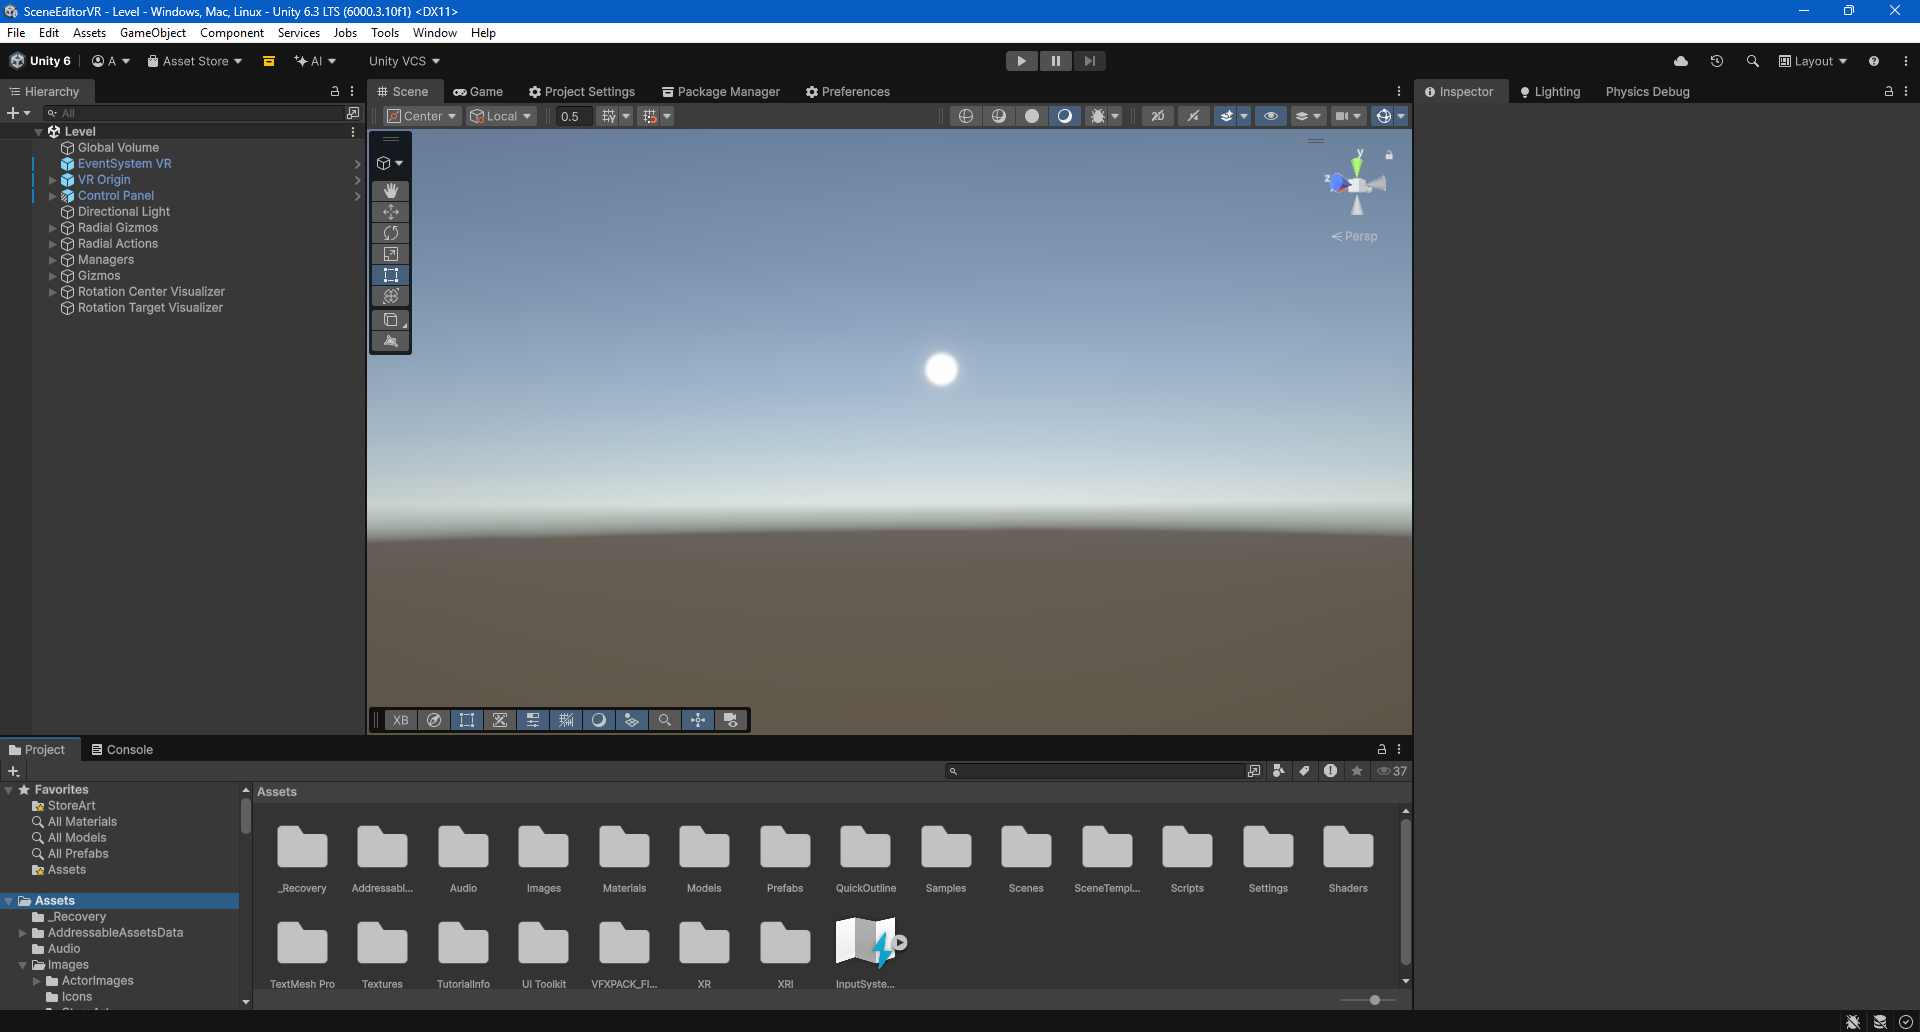
\includegraphics[width=\textwidth]{images/unity.png}
  \caption{Unity Desktop Editor}
  \label{fig:unity_desktop}
\end{figure}

The Unity Editor~\cite{UnityEngine2024} (Figure~\ref{fig:unity_desktop}) is the industry standard for XR development, utilizing a \textit{Scene View}.
Interaction within this environment is governed by the \textbf{WIMP} (Windows, Icons, Menus, Pointers) paradigm.
While highly precise, this interface creates a ``perceptual disconnect.'' Developers manipulate 3D spatial data
through a 2D monitor using a mouse, which lacks depth cues and physical scale.

Furthermore, the standard Unity workflow requires a repetitive cycle of ``editing'' and ``play-testing.''
Because the editor is not VR-native, the developer cannot stay within the immersive environment to make structural changes.
This results in a loss of \textit{flow state} and significant temporal overhead when fine-tuning the spatial ergonomics of a VR scene.

\subsection{Unreal Engine Scene Editor}

\begin{figure}[H]
  \centering
  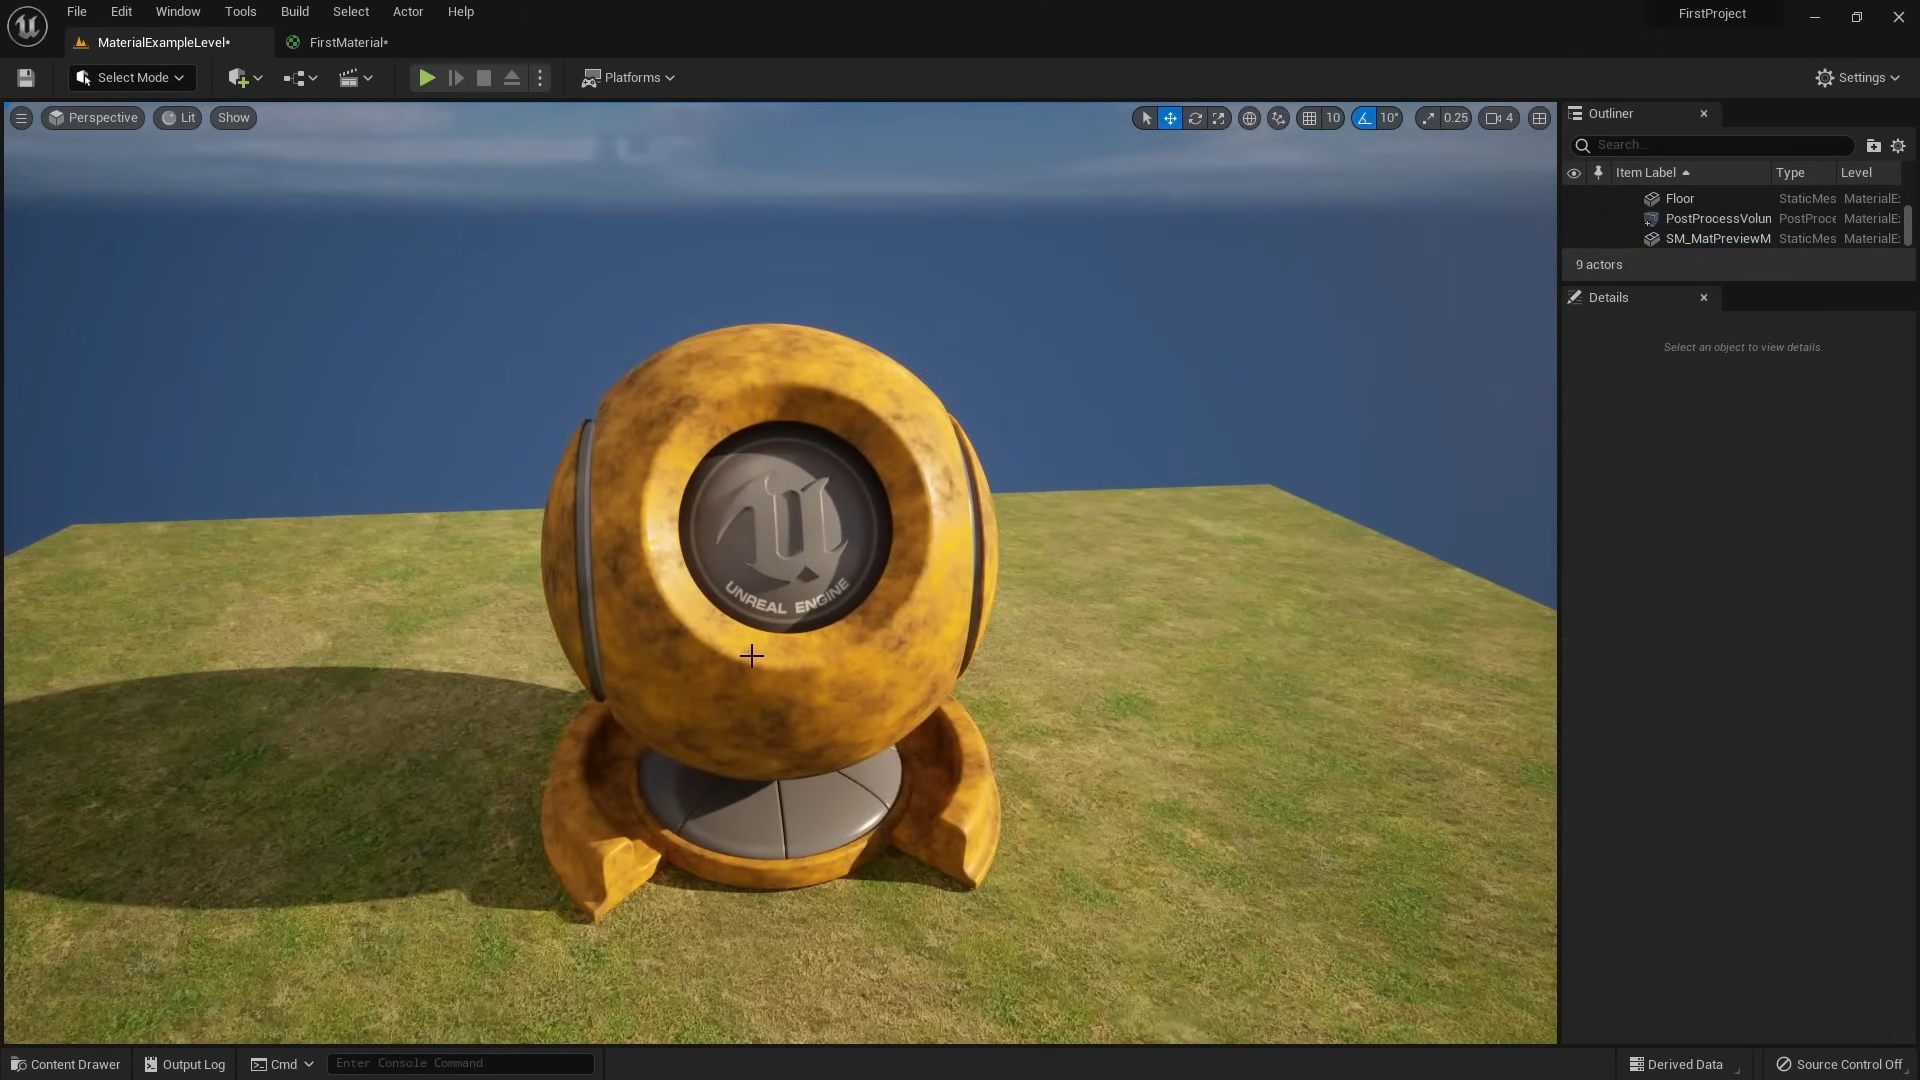
\includegraphics[width=\textwidth]{images/unreal.png}
  \caption{Unreal Desktop Editor}
  \label{fig:unreal_desktop}
\end{figure}

Unreal Engine~\cite{UnrealEngine2025} (Figure~\ref{fig:unreal_desktop}) represents the high-end of the XR development spectrum, offering robust tools for visual fidelity.
Historically, Epic Games attempted to bridge the 2D-3D gap with the introduction of the \textit{Unreal VR Editor} (Figure~\ref{fig:unreal_vr}) in 2016.
This tool enabled direct manipulation of the Scene Graph with 6DoF controllers and a floating world-space UI.

However, as the engine transitioned to Unreal Engine 5, this VR-native editing mode was largely sidelined in favor of
``VR Preview'' workflows. The industry consensus suggests that the original VR Editor failed to gain traction due to its
high cognitive load—it attempted to port a complex desktop-centric interface into a spatial environment without sufficient
simplification. This deprecation highlights a significant opportunity for specialized, lightweight authoring tools. Unlike the ``feature-heavy'' approach of Unreal, \textit{SceneEditorVR} prioritizes a streamlined UX, suggesting that immersive editing is more
effective when designed around spatial ergonomics rather than desktop-legacy menus.

\begin{figure}[H]
  \centering
  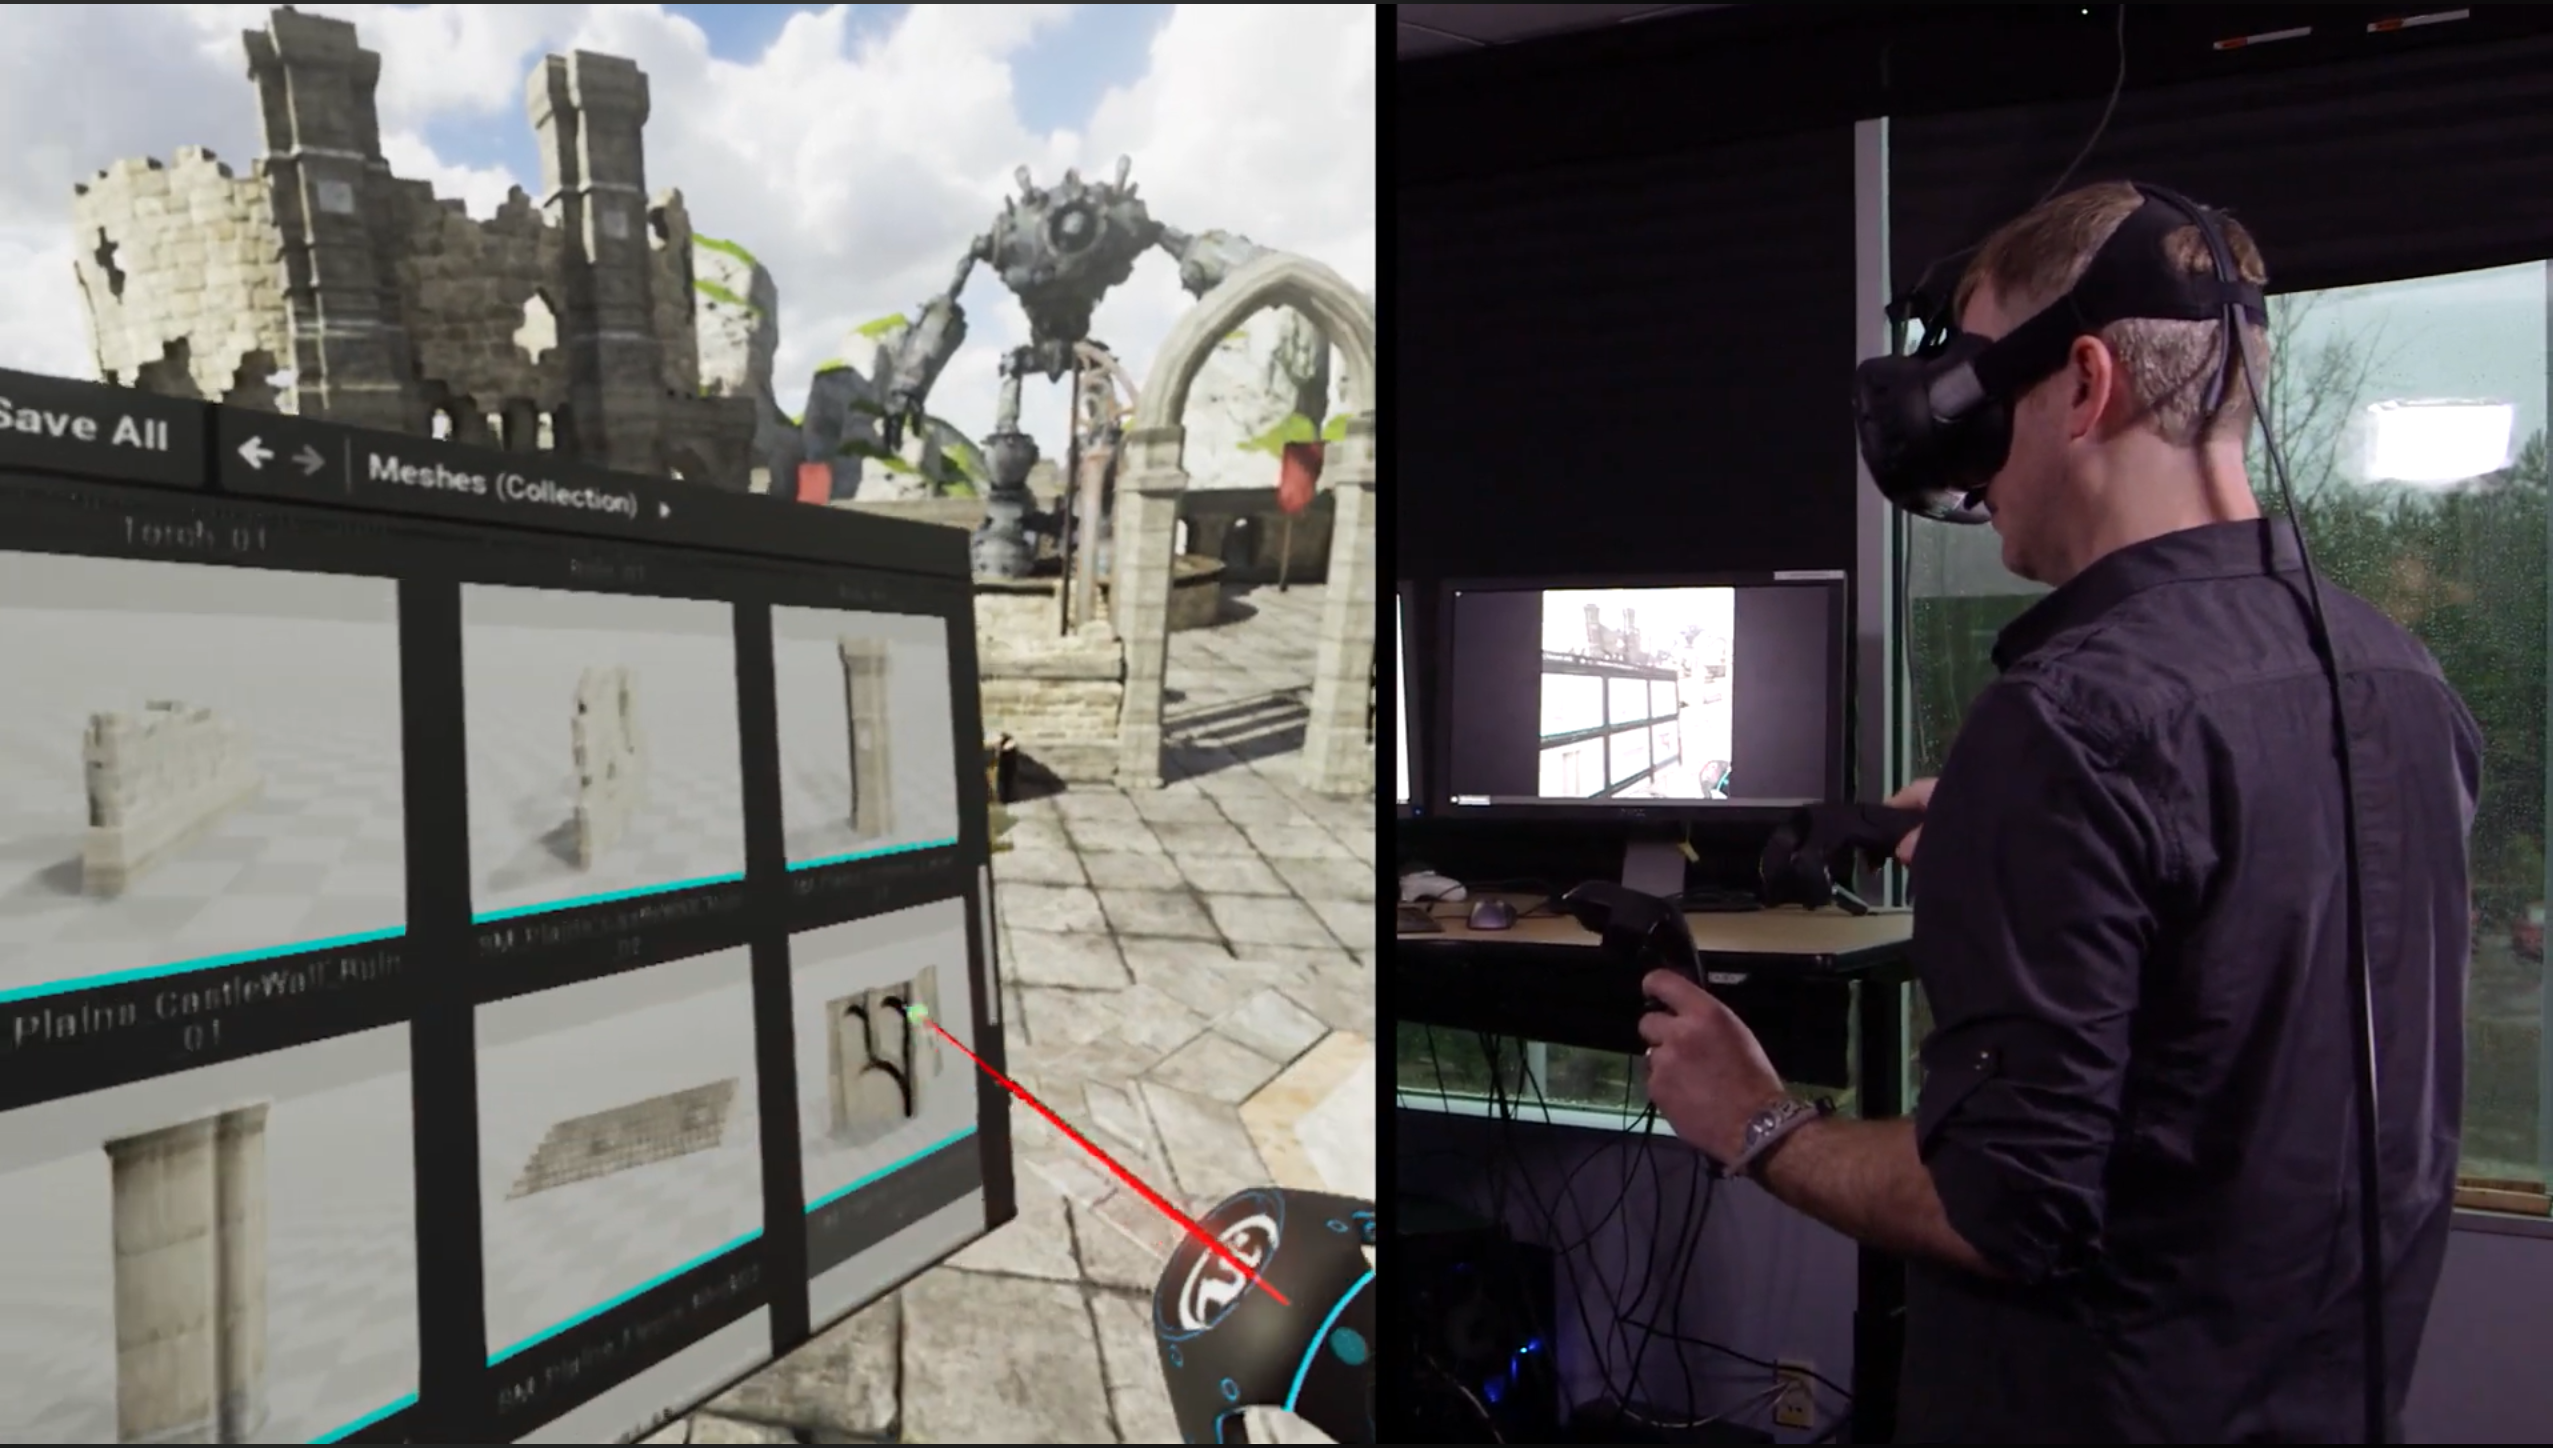
\includegraphics[width=\textwidth]{images/unreal_vr.png}
  \caption{Unreal VR Scene Editor~\cite{UnrealVREditor}}
  \label{fig:unreal_vr}
\end{figure}

\subsection{Godot Scene Editor}

\begin{figure}[H]
  \centering
  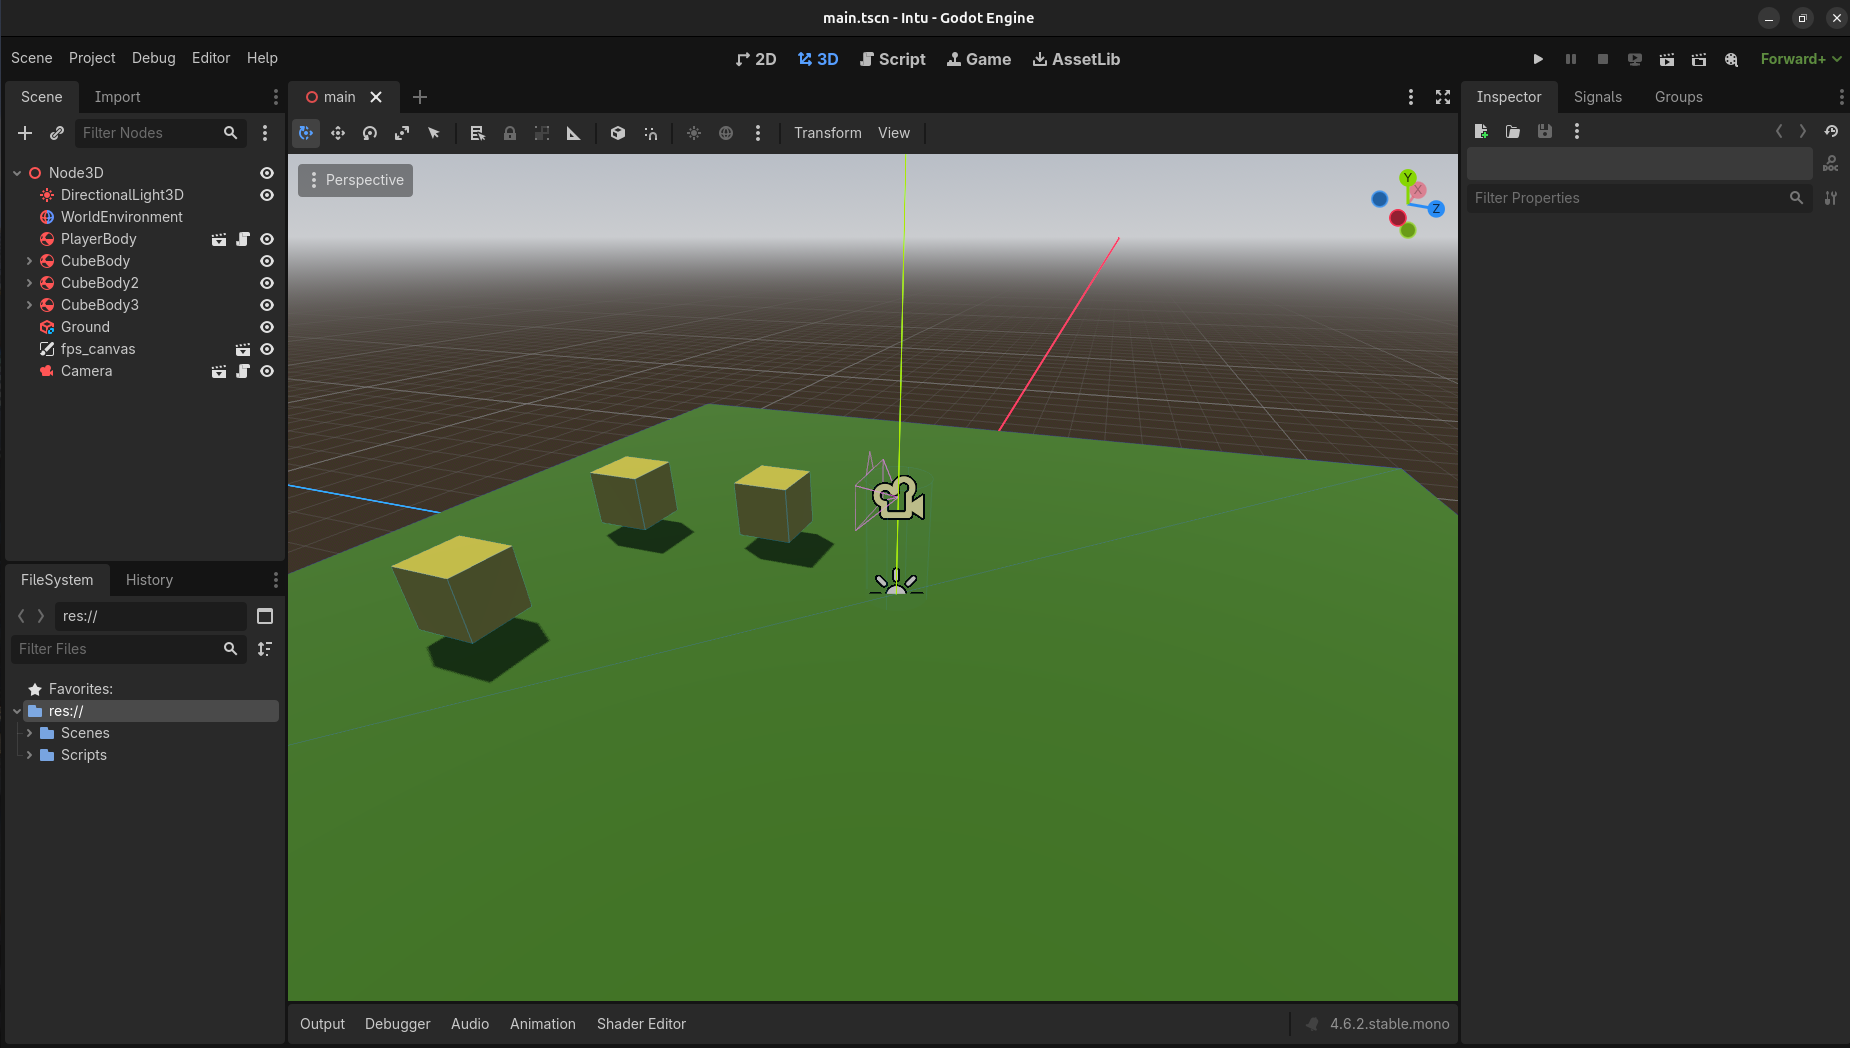
\includegraphics[width=\textwidth]{images/godot.png}
  \caption{Godot Desktop Editor}
  \label{fig:godot_desktop}
\end{figure}

Godot Engine~\cite{GodotEngine2026} (Figure~\ref{fig:godot_desktop}) offers a unique perspective on the evolution of immersive tools, as it is the only major engine to have
ported its full desktop editor to standalone VR hardware, specifically the Meta Quest series (Figure~\ref{fig:godot_vr}). In late 2024, the
Godot Editor was made available on the Horizon Store, allowing for a ``PC-less'' development workflow.

However, this implementation highlights the core thesis of this research: the \textit{spatial interaction gap}. While
the Godot editor runs natively on the headset, it remains a ``hybrid'' application. The interface is rendered as a 2D
floating window—a direct port of the WIMP-based Android version—rather than a native spatial environment.

This state of the art confirms that simply transporting 2D windows into a 3D space is insufficient. \textit{SceneEditorVR}
departs from this ``windowed'' approach by offering a ground-up spatial interface, prioritizing direct hand-object interaction
over traditional 2D menus.

\begin{figure}[H]
  \centering
  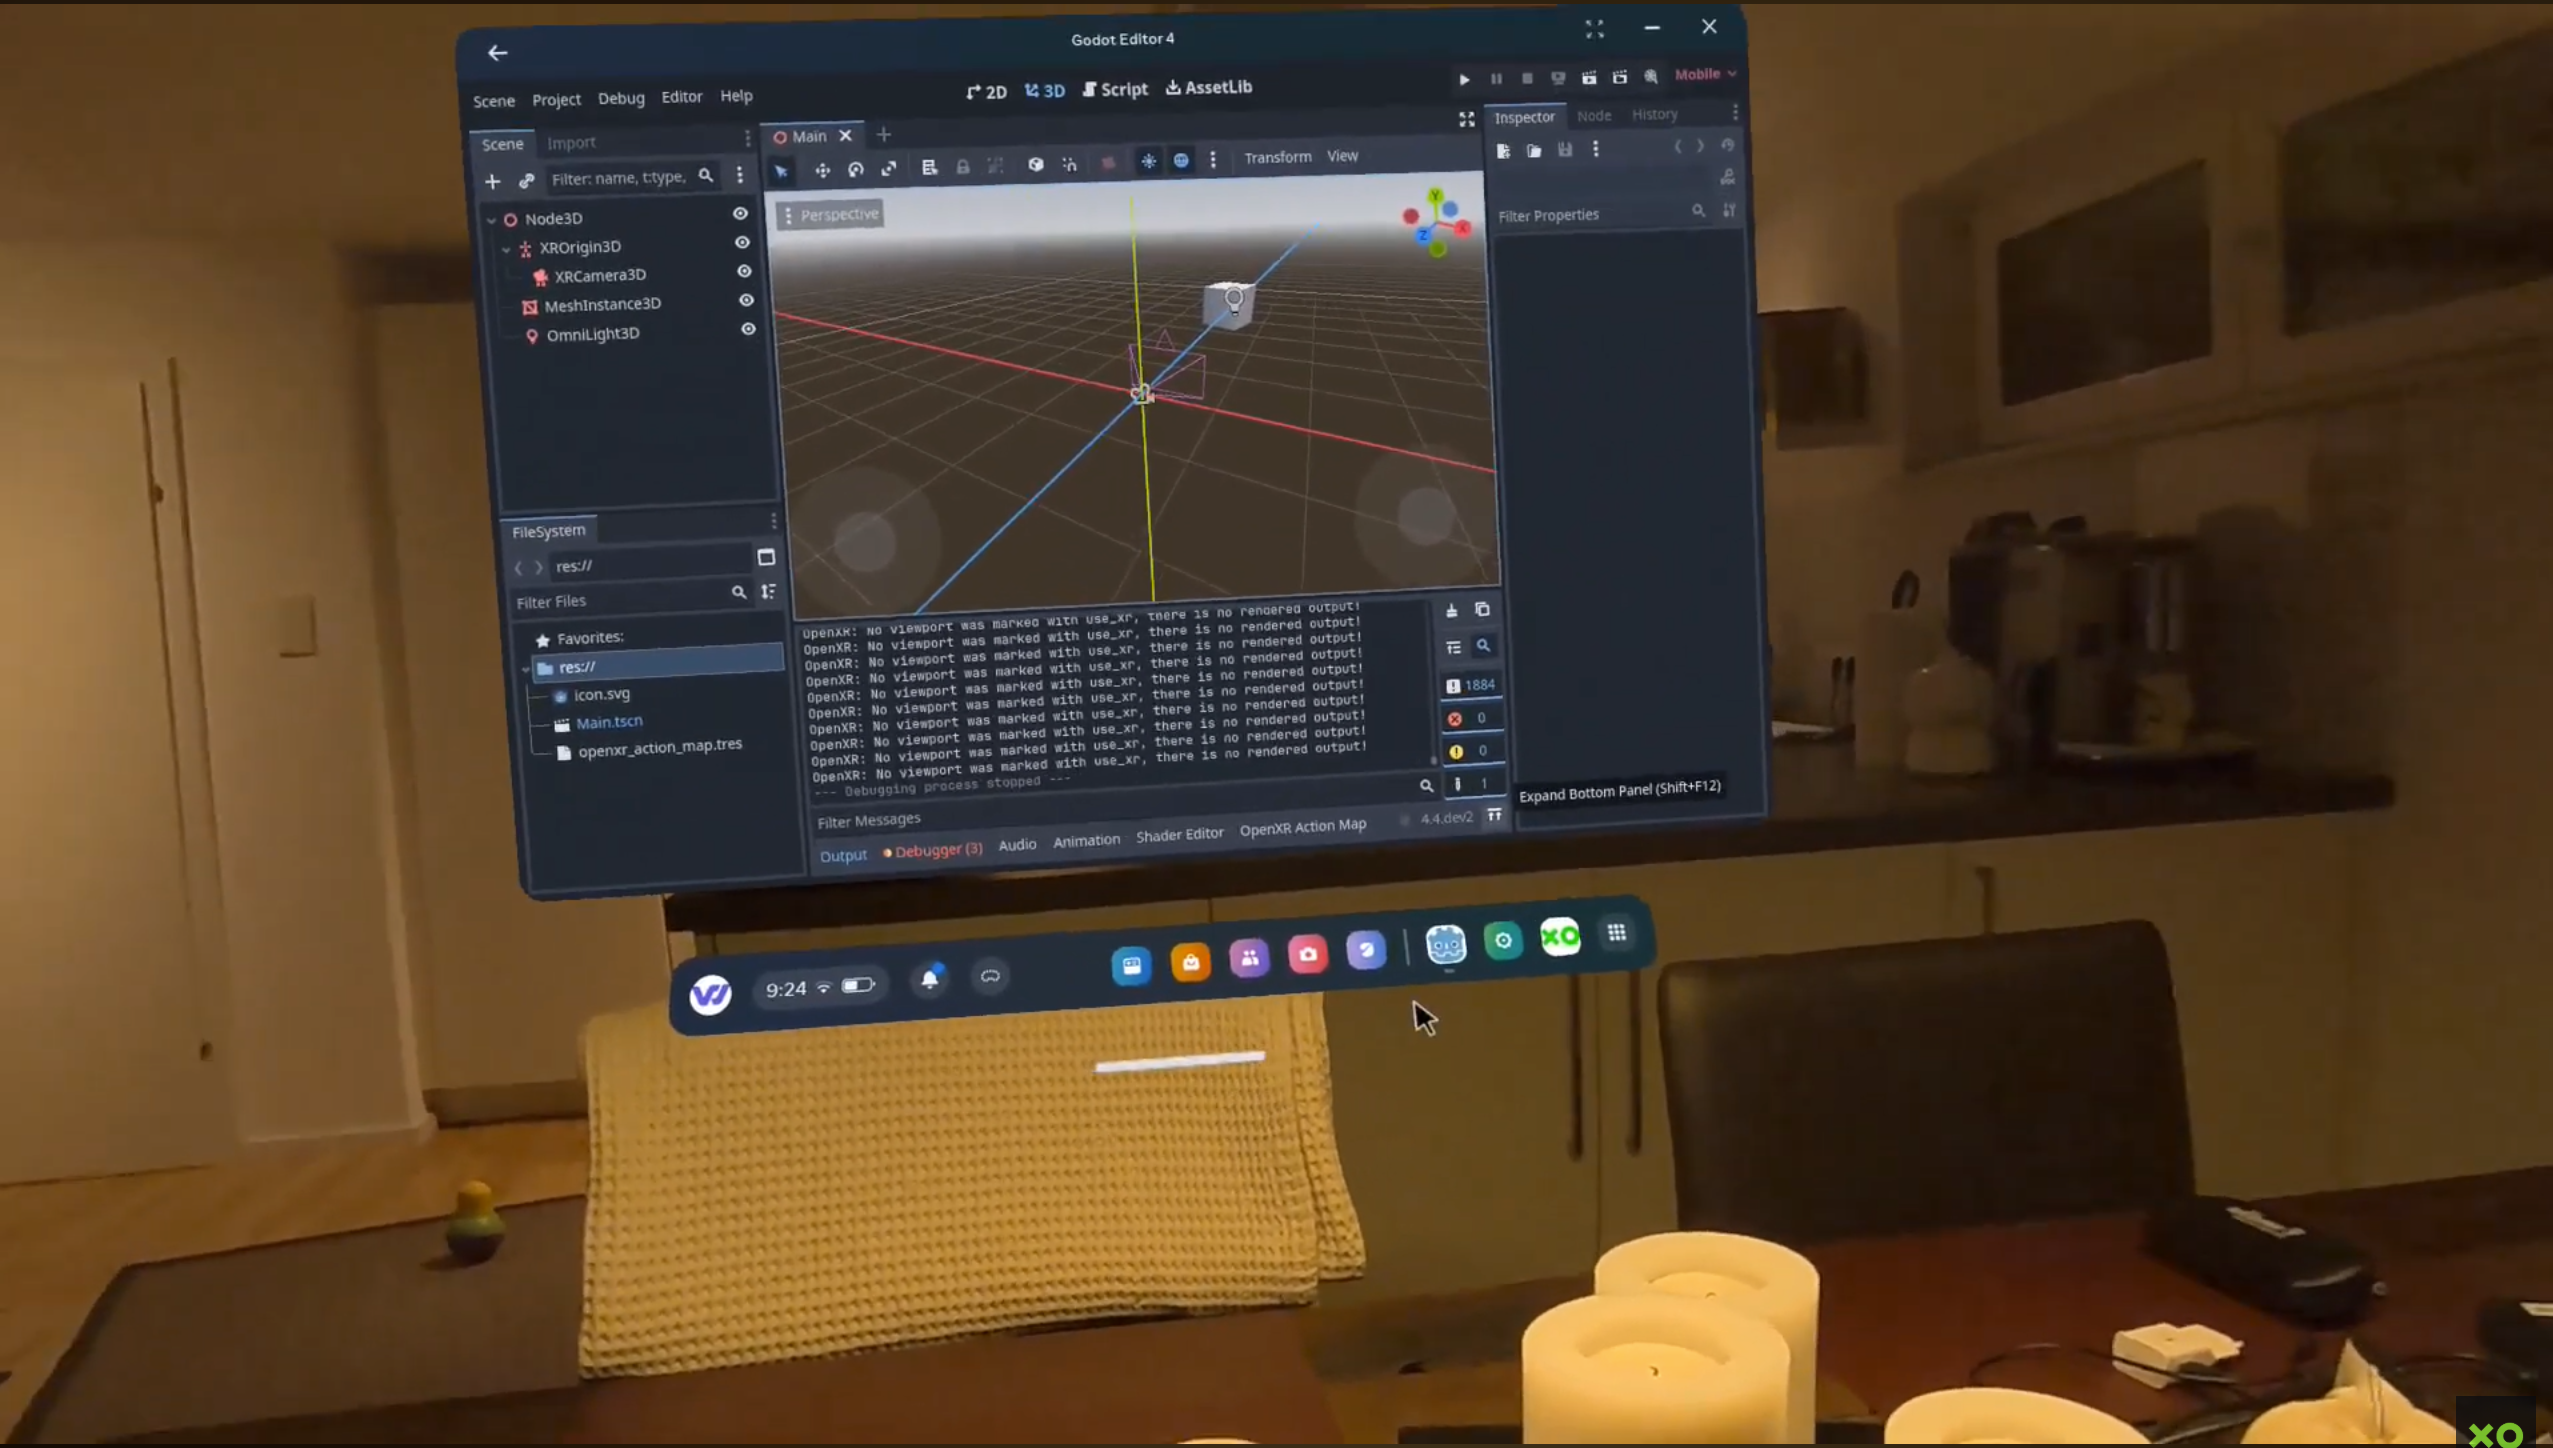
\includegraphics[width=\textwidth]{images/godot_vr.png}
  \caption{Godot Editor running in a Meta Quest~\cite{GodotEditorMetaQuest}}
  \label{fig:godot_vr}
\end{figure}

\section{VR-Native Scene Editors}

\subsection{Rec Room}

\begin{figure}[H]
  \centering
  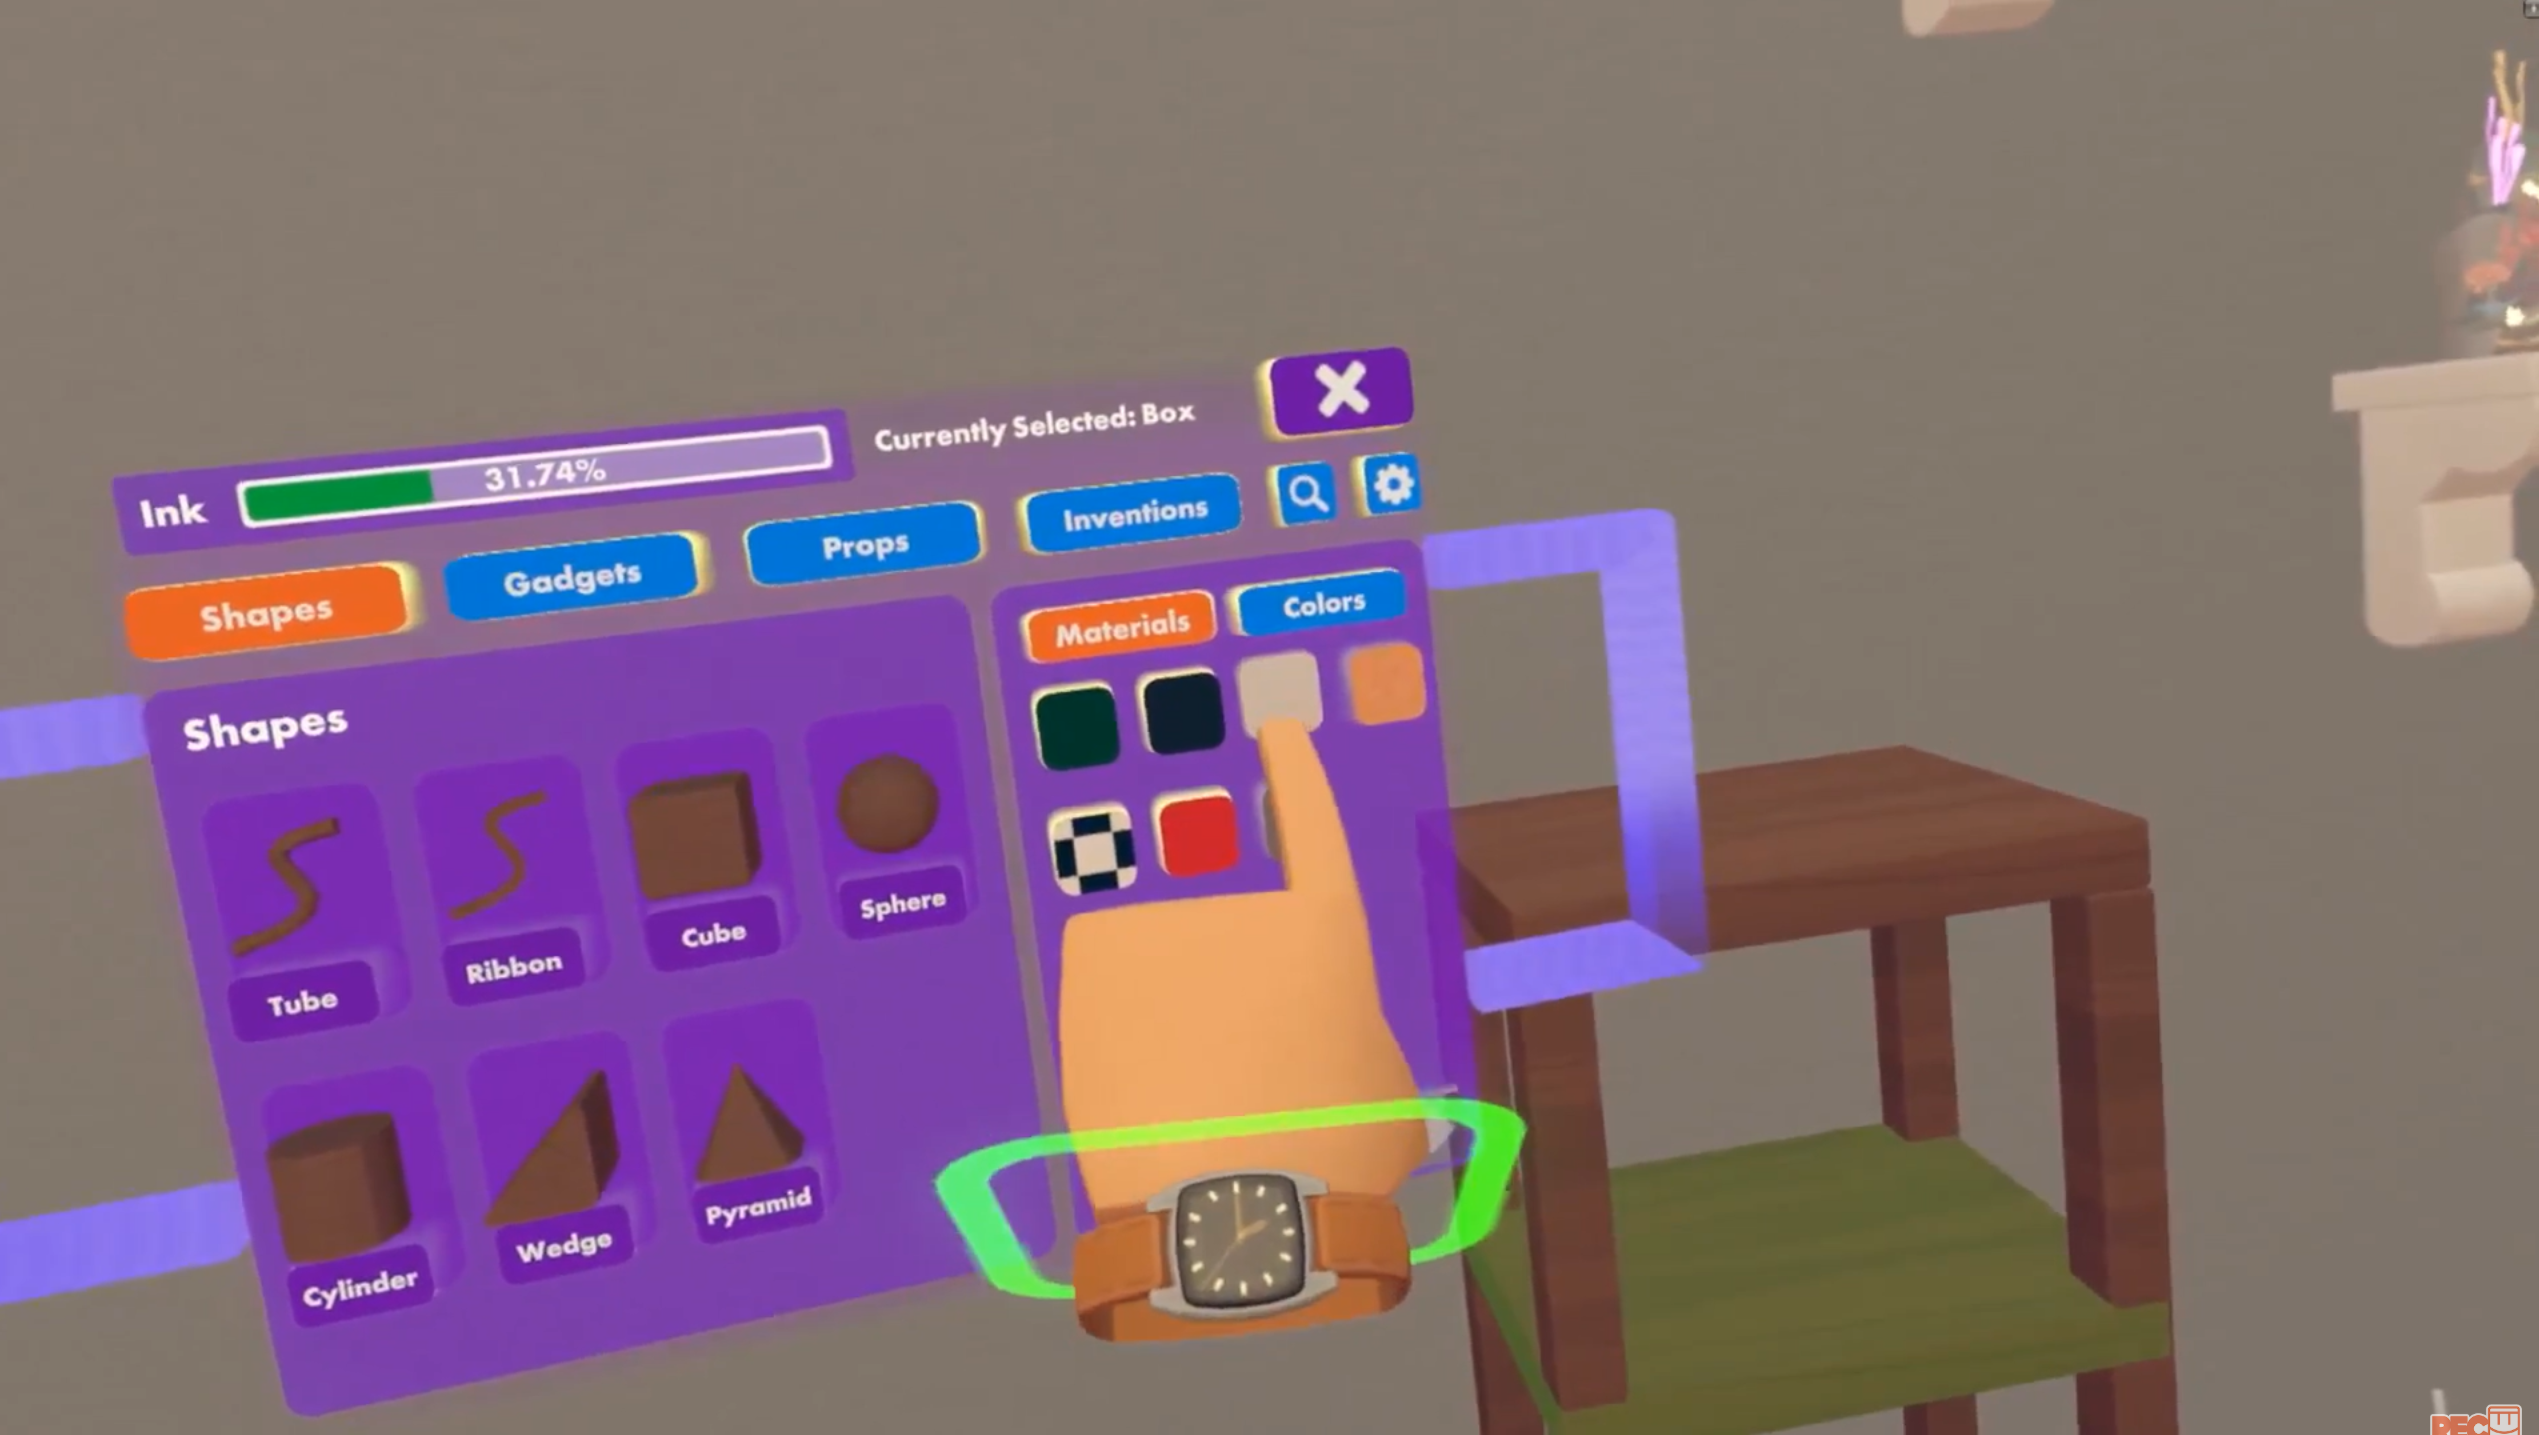
\includegraphics[width=\textwidth]{images/rec_room.png}
  \caption{Rec Room User Editor~\cite{RecRoom}}
  \label{fig:rec_room}
\end{figure}

Rec Room~\cite{RecRoom2016} (Figure~\ref{fig:rec_room}) represents the most successful implementation of a consumer-facing, VR-native creation system.
The primary interaction vector is the \textit{Maker Pen}, a multi-functional tool that enables users to
instantiate primitive geometry and place pre-defined assets within a shared 3D environment.

Key features of the Rec Room workflow relevant to \textit{SceneEditorVR} include:
\begin{itemize}
  \item \textbf{Diegetic Toolsets:} The use of a physical tool (the Maker Pen) to house UI menus reduces the cognitive load
        associated with navigating traditional ``flat'' menus.
  \item \textbf{Collaborative Design:} Rec Room allows multiple users to build in the same spatial viewport simultaneously,
        providing a real-time ``WYSIWYG'' (What You See Is What You Get) experience.
\end{itemize}

However, Rec Room is fundamentally a ``walled garden.'' Creations are restricted to the platform's proprietary format,
and the recent introduction of \textit{Rec Room Studio}—a desktop Unity plugin—suggests a pivot back to traditional
2D-based development for complex tasks. \textit{SceneEditorVR} addresses this by adopting the intuitive UX of the
Maker Pen while ensuring professional utility through open-source export capabilities.

\subsection{Arkio}

\begin{figure}[H]
  \centering
  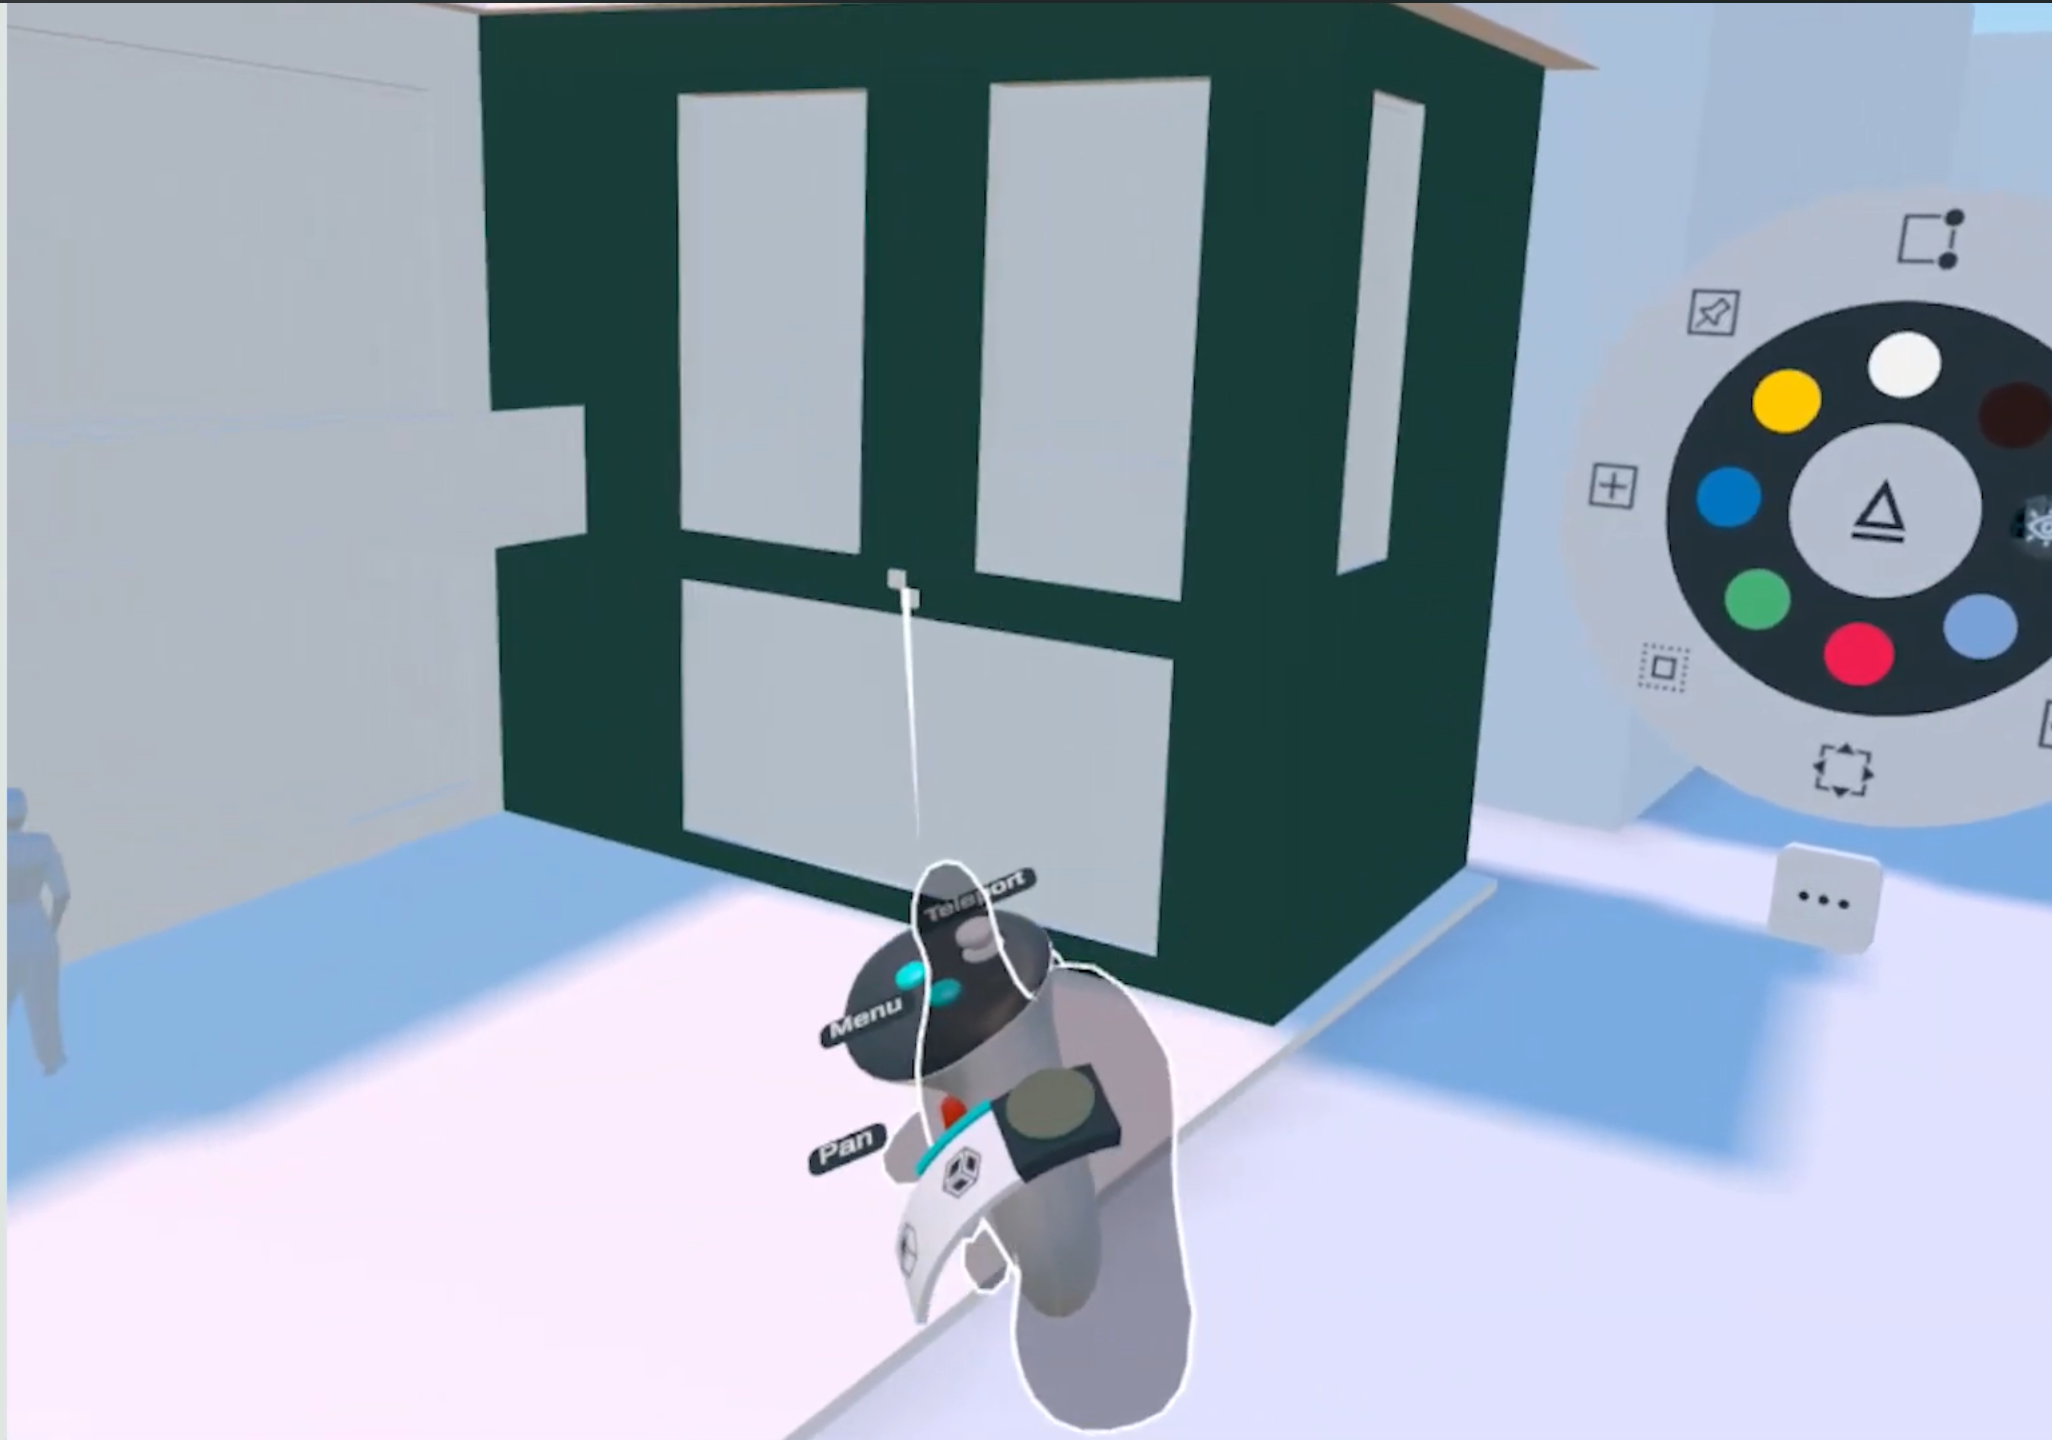
\includegraphics[width=\textwidth]{images/arkio.png}
  \caption{Arkio User Editor~\cite{Arkio}}
  \label{fig:arkio}
\end{figure}

Arkio~\cite{Arkio2026} (Figure~\ref{fig:arkio}) is a professional-grade collaborative design tool that bridges the gap between traditional architectural modeling and
immersive spatial design. Unlike gamified builders, Arkio is specifically engineered for AEC (Architecture, Engineering, and Construction)
professionals, allowing users to sketch building massing, move walls, and arrange furniture in a 1:1 scale environment.
It utilizes a unique volumetric modeling kernel that makes ``push-pull'' geometry manipulation feel intuitive with VR controllers,
effectively turning the virtual space into a digital version of physical model-making. For the purpose of this thesis,
Arkio serves as a critical example of an in-situ authoring tool that maintains professional utility through its
bidirectional integration with industry-standard software like Revit, Rhino, and Unity. This highlights that VR-native
editing is not merely for creative play but is a viable solution for high-precision spatial layout and rapid architectural prototyping.

\subsection{ShapesXR}

\begin{figure}[H]
  \centering
  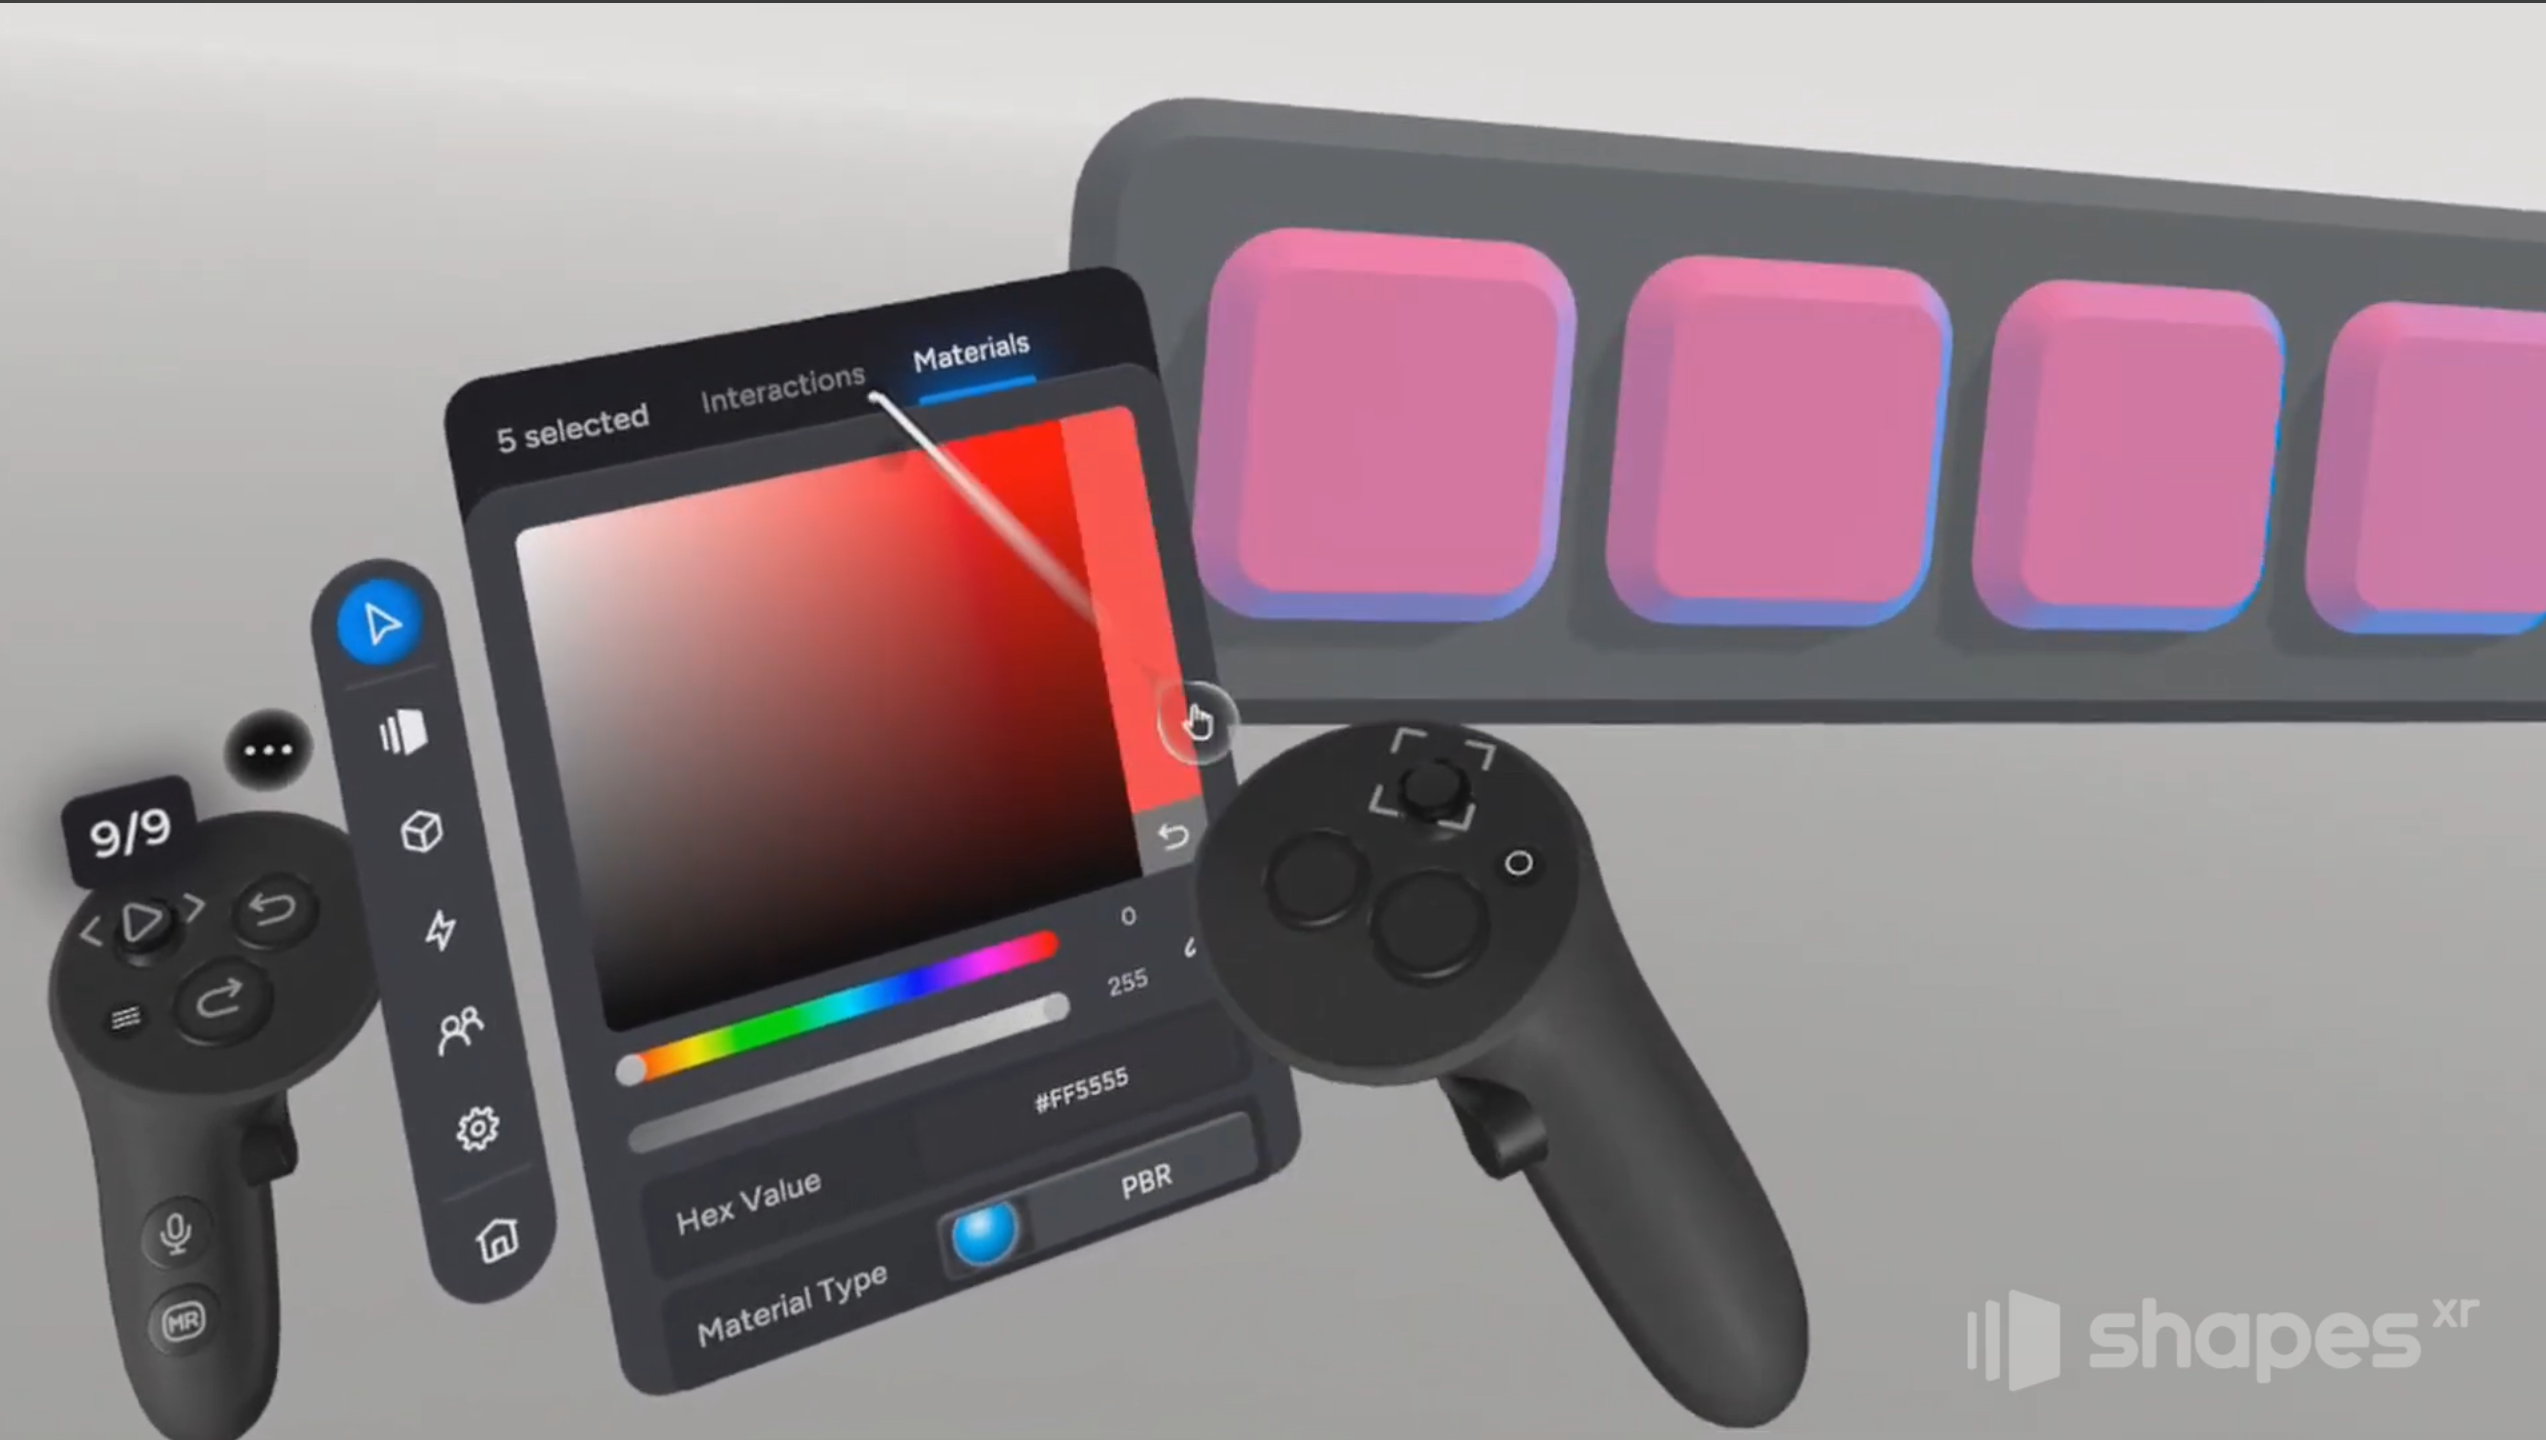
\includegraphics[width=\textwidth]{images/shapesxr.png}
  \caption{ShapesXR User Editor~\cite{ShapesXR}}
  \label{fig:shapesxr}
\end{figure}

ShapesXR~\cite{ShapesXR2026} (Figure~\ref{fig:shapesxr}) is an industry-standard prototyping platform designed to facilitate the transition from 2D concepts to 3D spatial interfaces.
It prioritizes low-fidelity ``gray-boxing'' over high-detail modeling, enabling UX designers to quickly block out user flows and
environmental layouts. A defining characteristic of ShapesXR is its ``Stages'' system—a spatial iteration of traditional
presentation slides—which allows creators to storyboard linear interactions within a 3D volume. By integrating with 2D design tools
like Figma and providing a dedicated Unity plugin for data handoff, ShapesXR validates the ``Rapid Prototyping'' objective of this research.
It demonstrates that the most effective VR authoring tools are those that simplify complex operations into intuitive spatial gestures,
allowing teams to iterate on the ``feel'' of an experience before committing to final production code.
\chapter{DESIGN}

\section{User Personas}

\subsection{Persona 1}

\subsubsection{Profile}

\begin{itemize}
  \item \textbf{Name}: Adam Smith
  \item \textbf{Age}: 26
  \item \textbf{Role}: Junior VR Developer
  \item \textbf{Background}: Adam has spent the last three years building VR environments
        for academic projects and small indie titles. He is technically proficient in Unity but often finds the
        ``monitor-and-mouse'' workflow creates a disconnect between his vision and the actual spatial feel of the VR scene.
\end{itemize}

\subsubsection{Technical Background}

\begin{itemize}
  \item \textbf{VR Experience}: Expert. Owns multiple headsets. Has hundreds of hours in VR across gaming, social VR, and development testing.
  \item \textbf{Game Editors}: Unity Power User. Comfortable with the Inspector and the Hierarchy structure.
  \item \textbf{Native VR Editors}: He has tried some applications with UGC (User Generated Content).
\end{itemize}

\subsubsection{Physical \& Environmental Context}

\begin{itemize}
  \item \textbf{Physical Health}: Normal. No history of motion sickness (strong ``VR legs''). He can tolerate long sessions
        in the headset without discomfort.
  \item \textbf{Physical Setup}: Large room-scale boundary (3x3m). Prefers standing while working to reach high or low within the virtual space.
\end{itemize}

\subsubsection{Psychographic \& Goals}

\begin{itemize}
  \item \textbf{Goal}: To rapidly block out a scene's layout while standing inside it,
        ensuring that the scale of the furniture and objects feels ``correct'' to a human player immediately.
  \item \textbf{Pain Points}: He hates having to take the headset off, adjust an object by 5cm in Unity on his monitor,
        and put the headset back on to check the result.
  \item \textbf{Expectations}: He expects high precision. He won't be satisfied with ``loose'' placements; he requires transform
        snapping and multi-selection to feel like he is in a professional environment.
\end{itemize}

\subsubsection{User Story}

The goals of this persona reflect a desire for workflow continuity: ``As a developer who spends all day in Unity, I want a tool that allows me to manipulate 3D assets with the same precision as
my keyboard and mouse, but with the spatial intuition that only VR provides. I want to build the ``bones'' of my level while standing
inside it so I don't have to guess the scale anymore.''

\subsection{Persona 2}

\subsubsection{Profile}

\begin{itemize}
  \item \textbf{Name}: Rachel Pierce
  \item \textbf{Age}: 23
  \item \textbf{Role}: Digital Artist
  \item \textbf{Background}: Rachel is an active member of the social VR and modding communities.
        While she has a natural eye for interior design and 3D composition, she finds professional game engines
        like Unity intimidating and overly technical. She prefers ``in-game'' creative tools that allow for immediate visual feedback.
\end{itemize}

\subsubsection{Technical Background}

\begin{itemize}
  \item \textbf{VR Experience:} High (Uses VR daily for social interaction and world exploration).
  \item \textbf{Game Editors:} None (Has no experience with professional Game Engines).
  \item \textbf{Prototyping Tools:} Expert in UGC (The Sims Build Mode, Animal Crossing, and basic Blender for asset preparation).
  \item \textbf{VR Creation Apps:} Moderate (Frequent user of Rec Room Maker Pen and VRChat Home editors).
\end{itemize}

\subsubsection{Physical \& Environmental Context}

\begin{itemize}
  \item \textbf{Physical Health}: Normal. However, she is prone to slight ``simulator sickness'' during rapid artificial movement,
        making stable locomotion and snap turning essential for her comfort.
  \item \textbf{Physical Setup}: Stationary/Small room setup. She relies on in-game vertical and horizontal
        locomotion because her physical play area is limited.
\end{itemize}

\subsubsection{Psychographic \& Goals}

\begin{itemize}
  \item \textbf{Goal}: To intuitively design aesthetically pleasing 3D dioramas and room layouts without needing to learn complex engine logic.
  \item \textbf{Pain Points}: She feels limited by the ``walled gardens'' of social VR apps; she wants a simple tool where she can create a
        scene and actually own the resulting file (exporting).
  \item \textbf{Expectations}: She expects a clean, non-distracting interface and a ``Creative Mode'' feel that prioritizes
        visual clarity over technical data.
\end{itemize}

\subsubsection{User Story}

The core motivation for this persona centers on accessibility: ``As a creative hobbyist who loves designing spaces, I want an accessible VR tool that functions like a high-end building game.
I want to pick items from a library and snap them together in 1:1 scale, and then be able to export my work as a standard 3D file
to share with my friends or use in my digital art portfolio.''

\section{Movement System}
The navigation system in SceneEditorVR is designed to provide the user with full six-degrees-of-freedom (6DoF) mobility, allowing for
precise positioning within the 3D environment. The choice of locomotion methods was driven by the need for fluid movement that
does not interrupt the creative workflow.

\subsection{Horizontal Plane Movement}
Horizontal movement is implemented via Smooth Locomotion, mapped to the left controller’s thumbstick. While many VR applications
utilize ``Teleportation'' to minimize physical discomfort, it was found to be too disjointed or cumbersome for a scene-editing
context. To justify this choice, the target audience for the application was identified as
experienced VR users. By assuming a high level of ``VR habituation,'' the design prioritizes continuous, precise spatial translation
over the comfort-centric limitations of teleportation.

\subsection{Vertical Movement}
To facilitate vertical exploration and the placement of assets at varying heights (e.g., ceiling fixtures or multi-level structures),
a dedicated vertical translation system was implemented using the controller Grip buttons. Pressing the left grip initiates an upward ascent,
while the right grip initiates a descent. This ``button-mapped'' approach was chosen after initial testing of ``air-grabbing'' or ``world-pulling''
mechanics proved to be unintuitive for users during long editing sessions. By decoupling verticality from hand gestures, the user maintains
a stable viewpoint while adjusting their elevation.

\subsection{Rotation}
Rotational navigation is handled through Snap Turning on the right thumbstick. By flicking the stick left or right, the user’s view
rotates by a fixed degree increment. This was selected as it remains the industry standard for VR orientation; it provides the necessary
change in perspective required to view a 3D model from all sides while significantly reducing the risk of motion sickness
compared to smooth, continuous rotation.
\section{Assets Interaction}
In \textit{SceneEditorVR}, users interact with environmental assets by targeting them directly using the controllers' selection rays. The interaction system supports both single-object and multi-object selection, allowing users to manipulate multiple assets simultaneously. Once selected, assets can be modified through the activation of spatial transformation gizmos or through contextual actions such as duplication and deletion. When a multi-selection is active, the system dynamically calculates a shared center of mass (pivot point) from all selected objects, serving as the central anchor for subsequent translation, rotation, and scaling operations.
\section{Gizmos}
When an asset is selected, one of three possible transformation gizmos can be activated (Figures~\ref{fig:translation_gizmo}, \ref{fig:rotation_gizmo}, and \ref{fig:scale_gizmo}):

\subsection{Translation Gizmo}

\begin{figure}[H]
  \centering
  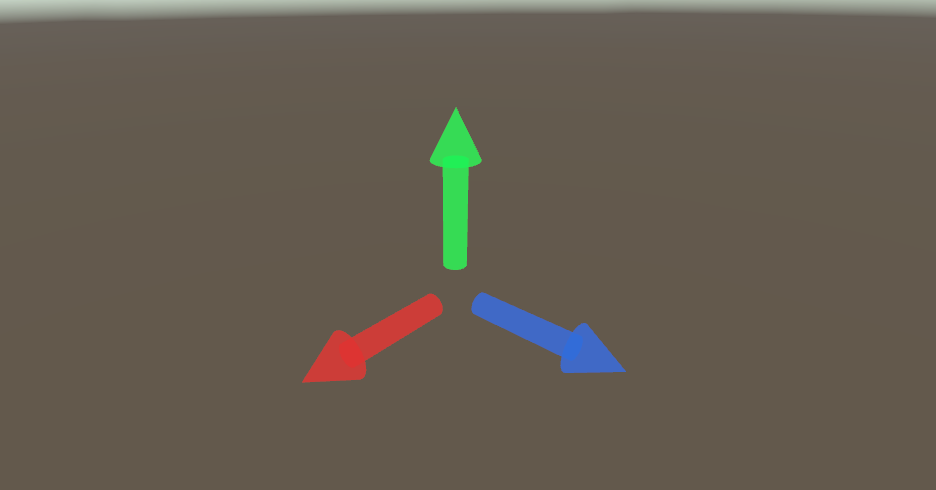
\includegraphics[width=\textwidth]{images/move_gizmo.png}
  \caption{Translation Gizmo}
  \label{fig:translation_gizmo}
\end{figure}

The translation gizmo consists of three arrows, one corresponding to each axis. The user can interact with the arrows to move the assets along each axis.

\subsection{Rotation Gizmo}

\begin{figure}[H]
  \centering
  
\includegraphics[width=\textwidth]{images/rotation_gizmo.png}
  \caption{Rotation Gizmo}
  \label{fig:rotation_gizmo}
\end{figure}

The rotation gizmo features three rotational rings, one for each axis. The user can interact with the rotators to rotate the assets around each axis.

\subsection{Scale Gizmo}

\begin{figure}[H]
  \centering
  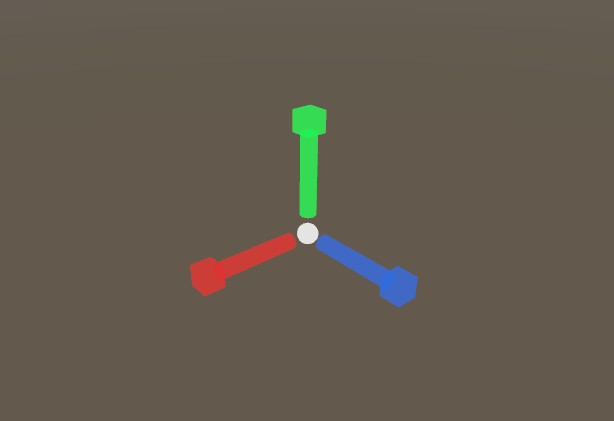
\includegraphics[width=\textwidth]{images/scale_gizmo.png}
  \caption{Scale Gizmo}
  \label{fig:scale_gizmo}
\end{figure}

The scale gizmo incorporates three scaling handles, one for each axis. The user can interact with the scalers to scale the assets in each axis. Additionally, it features a central white sphere that enables uniform scaling across all three axes.

\section{Radial Menus}

The application utilizes two button-activated radial menus (Figures~\ref{fig:radial_actions} and \ref{fig:radial_transform}) designed to streamline high-frequency
tasks through rapid, fluid interactions. To operate them, the user holds the designated button
and gestures toward an option, confirming their choice instantly upon release. This intuitive
selection method was specifically chosen to minimize friction for the actions performed most often.

\subsection{Actions Radial Menu}

\begin{figure}[H]
  \centering
  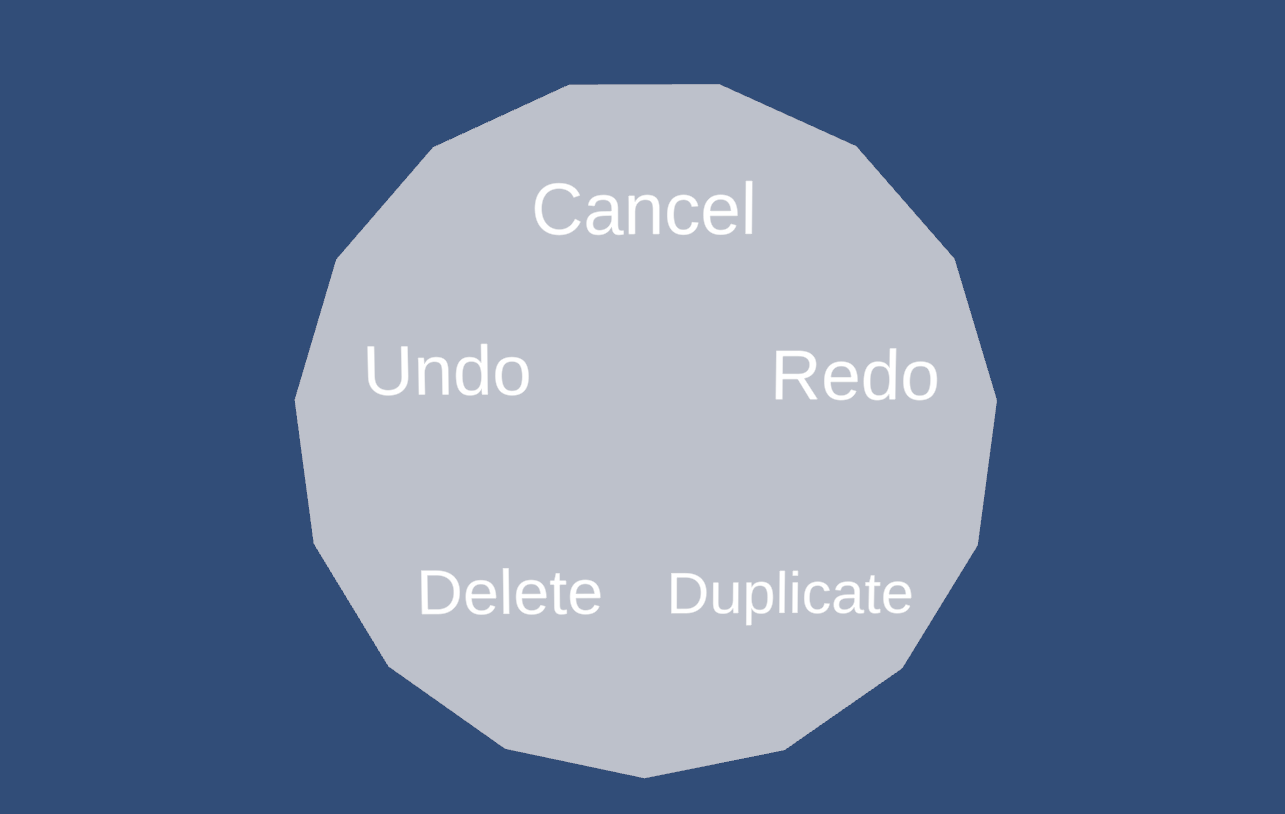
\includegraphics[width=\textwidth]{images/radial_actions.png}
  \caption{Actions Radial Menu}
  \label{fig:radial_actions}
\end{figure}

The actions radial menu contains the following options:
\begin{itemize}
  \item \textbf{Cancel}: Cancels any pending actions.
  \item \textbf{Redo}: Redoes the last undone action.
  \item \textbf{Duplicate}: Duplicates the currently selected assets.
  \item \textbf{Delete}: Deletes the currently selected assets.
  \item \textbf{Undo}: Undoes the last action.
\end{itemize}

\subsection{Transform Radial Menu}

\begin{figure}[H]
  \centering
  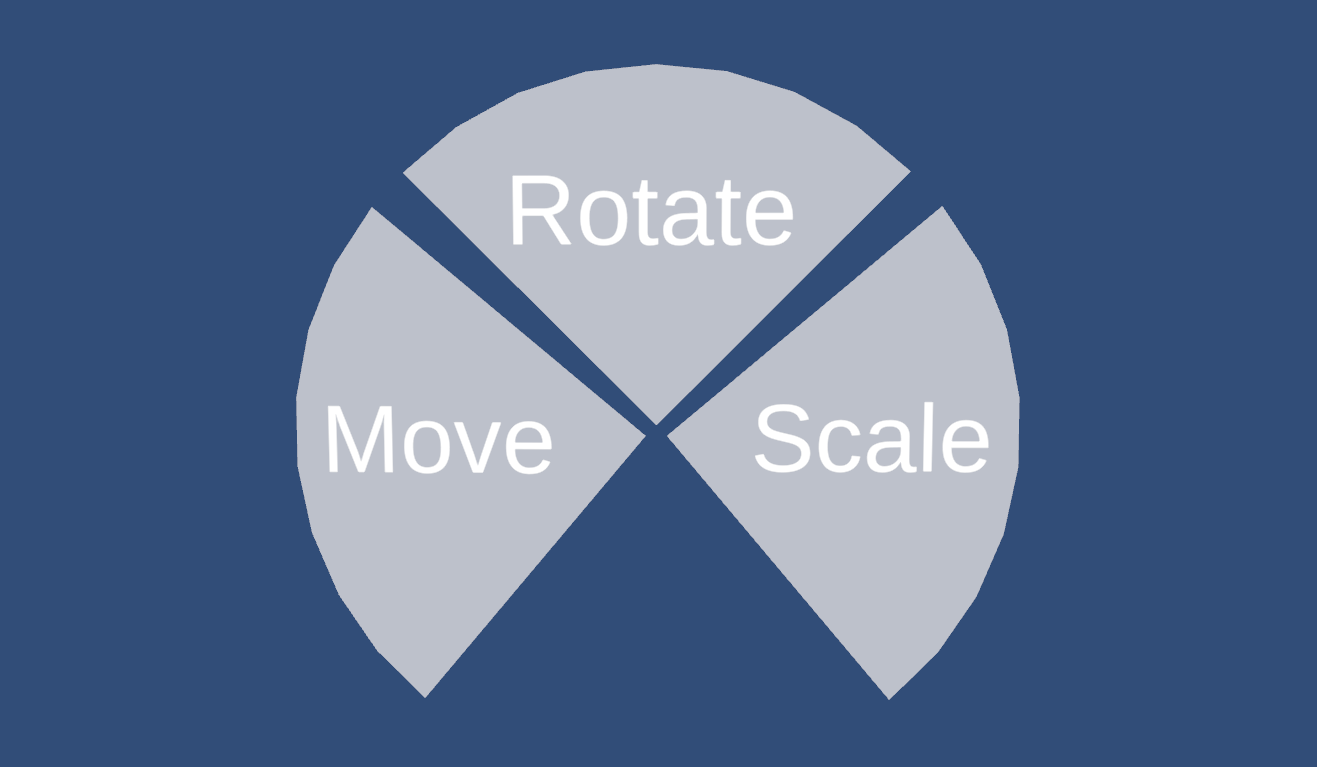
\includegraphics[width=\textwidth]{images/radial_transform.png}
  \caption{Transform Radial Menu}
  \label{fig:radial_transform}
\end{figure}

The transform radial menu contains the following options:
\begin{itemize}
  \item \textbf{Move}: Activates the translation gizmo for positional adjustments.
  \item \textbf{Rotate}: Activates the rotation gizmo for angular adjustments.
  \item \textbf{Scale}: Activates the scale gizmo for resizing adjustments.
\end{itemize}

\section{Control Panel}

\begin{figure}[H]
  \centering
  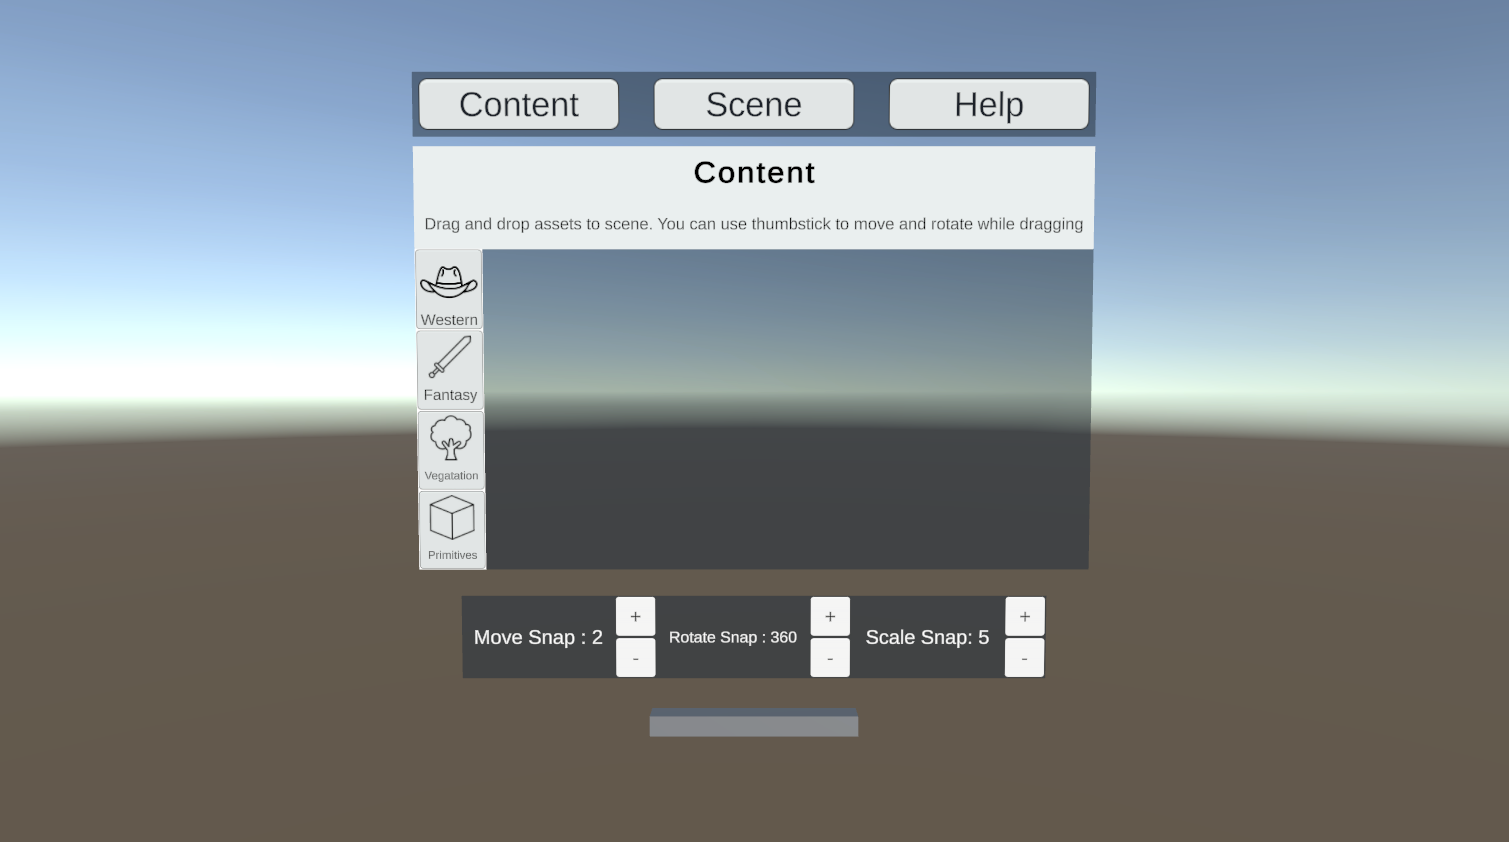
\includegraphics[width=\textwidth]{images/control_panel.png}
  \caption{Control Panel}
  \label{fig:control_panel}
\end{figure}

The level editor features a central control panel (Figure~\ref{fig:control_panel}) modeled after the Meta Horizon OS interface. This panel can be freely
repositioned within the environment or instantly recalled to the user's position using the Settings button.

\subsection{Content Tab}

\begin{figure}[H]
  \centering
  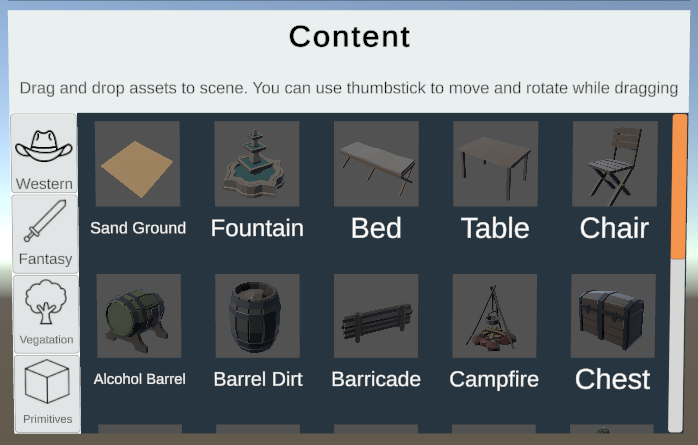
\includegraphics[width=\textwidth]{images/content_tab.png}
  \caption{Content tab in the Control Panel}
  \label{fig:content_tab}
\end{figure}

This tab (Figure~\ref{fig:content_tab}) serves as a library for all predefined assets available for use in the scene.

\subsection{Scene Tab}

\begin{figure}[H]
  \centering
  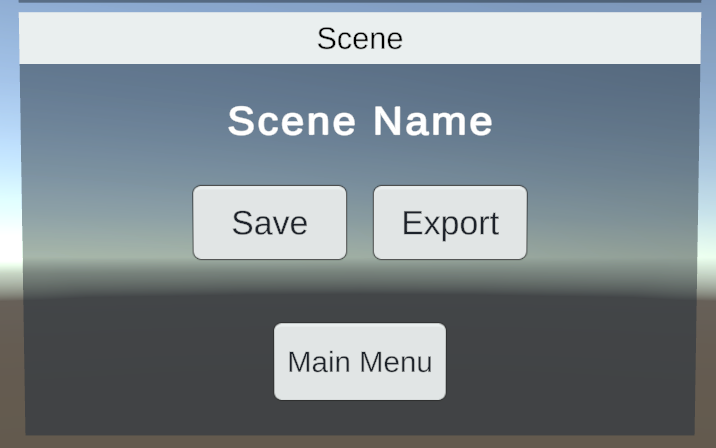
\includegraphics[width=\textwidth]{images/scene_tab.png}
  \caption{Scene tab in the Control Panel}
  \label{fig:scene_tab}
\end{figure}

The Scene tab (Figure~\ref{fig:scene_tab}) provides essential management tools, allowing users to save their progress, export the
current scene, or exit to the main menu.

\subsection{Help Tab}

\begin{figure}[H]
  \centering
  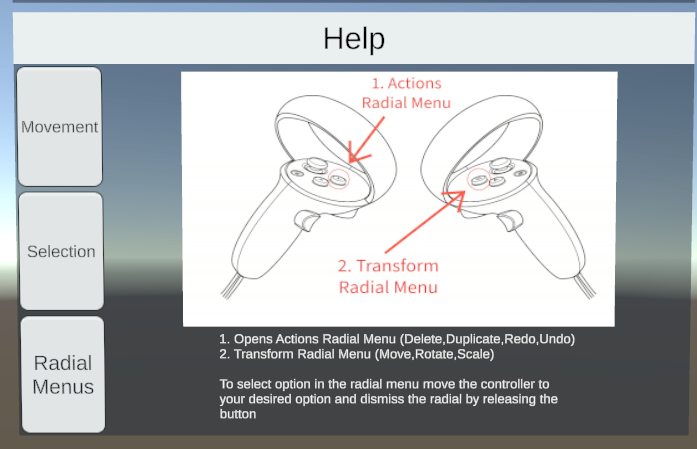
\includegraphics[width=\textwidth]{images/help_tab.png}
  \caption{Help tab in the Control Panel}
  \label{fig:help_tab}
\end{figure}

The Help tab (Figure~\ref{fig:help_tab}) contains detailed documentation and reference material regarding the application's controls.

\section{Assets}

The application utilizes a selection of predefined assets for two primary reasons. First, implementing custom asset
creation or import pipelines was deemed outside the technical scope of this thesis. Second, providing a curated library aligns
with the design philosophy of established User-Generated Content (UGC) platforms and the Unreal VR Editor. This approach reduces
the designer's overhead, allowing them to focus exclusively on environmental composition and level design.

To facilitate organized browsing, the assets are categorized into the following themed sections:

\begin{itemize}
  \item \textbf{Western:} Thematic elements and structures for frontier-style environments.
  \item \textbf{Medieval:} Architectural components and props for historical or fantasy settings.
  \item \textbf{Vegetation:} Natural assets including trees, shrubs, and flora.
  \item \textbf{Primitive Objects:} Basic geometric shapes used for prototyping and structural block-outs.
\end{itemize}

\section{Rotation}

Unlike traditional desktop-based 3D editors that map 2D mouse coordinates to 3D rotation axes, SceneEditorVR
leverages the six degrees of freedom (6-DOF) inherent in Virtual Reality. A custom Spatial Rotation
Visualizer was developed to make angular manipulation more intuitive. Upon selecting a rotation axis, the system instantiates two components:
a static Center Anchor and a dynamic Target Visualizer. The software calculates the angular displacement
of the VR controller relative to the center anchor in real-time. By mapping the object’s orientation to the vector formed between
these two visualizers, the user can ``steer'' the asset. This creates a direct 1:1 spatial mapping where the asset’s final orientation
aligns precisely with the user’s physical pointing direction.

\section{Snapping}

One of the inherent challenges of 3D UI design is the lack of tactile feedback, which can make precise alignment difficult for the user.
To mitigate this, SceneEditorVR utilizes a Discrete Transformation Toggle (Snapping). This feature provides a ``magnetic'' feel to asset
placement, allowing users to align objects with mathematical accuracy despite the inherent jitter of handheld VR controllers. The
interface offers granular control, enabling users to define the ``snap-step'' for translation, rotation, and scale. For workflows
requiring organic or high-fidelity placement, the snapping constraints can be bypassed by setting the increments to zero. By
integrating this system into the drag-and-drop workflow, the application reduces the need for secondary ``corrective'' transformations.

\section{Drag And Drop}

To streamline the scene composition workflow, SceneEditorVR implements a seamless transition between asset instantiation and placement.
Drawing inspiration from industry-standard game engines, the system utilizes a drag-and-drop paradigm from a centralized content panel.
To reduce task completion time a Hybrid Transformation Model was introduced: while an asset is being ``held'' in the drag state, the user
can utilize the controller’s thumbstick for coarse adjustments. This allows for simultaneous translation and rotation before
the user commits to the final position, effectively decoupling rapid spatial orientation from the high-precision refinements provided
by the gizmo system.

\chapter{IMPLEMENTATION}

\section{Tech Stack}

\subsection{Game Engine}

While developing a proprietary engine was initially considered, it was deemed outside the scope of this research.
Consequently, Unity was selected as the primary development platform due to its extensive documentation and proven track record
in deploying high-performance Virtual Reality applications. Unreal Engine was excluded due to its significantly higher hardware overhead
and resource requirements for standalone mobile VR deployment. Furthermore, while Godot is an emerging open-source alternative,
it was determined that its XR toolset currently lacks the production maturity required for the seamless,
high-fidelity VR interactions intended for this project.

\subsection{Use of Unity SDKs}

A deliberate architectural decision was made to avoid high-level frameworks such as the Meta XR SDK or the Unity XR Interaction Toolkit.
While these SDKs provide rapid prototyping capabilities, they often introduce significant software overhead and unnecessary dependencies
that can complicate the project's lifecycle. By implementing a custom interaction system, the application maintains a lightweight footprint
and ensures better long-term maintainability. Furthermore, this ``low-level'' approach minimizes engine-specific abstractions, facilitating
a more straightforward porting process to other platforms or engines by reducing reliance on proprietary black-box components.

\section{Interaction System}

\subsection{Interactables}

A custom interaction framework was developed to manage the relationship between the user's rays and the objects.
This system is built upon a base class, \texttt{Interactable}, which implements a Finite State Machine (FSM)
to track the lifecycle of an interaction. By using an inheritance-based model, specific behaviors are decoupled from the core state logic.

The \texttt{Interactable} class manages five distinct states that define the object's availability and current engagement level:

\begin{itemize}
  \item \textbf{IE\_INACTIVE}: The object is functionally disabled. Raycasts are ignored, and no interaction logic is processed.
  \item \textbf{IE\_IDLE}: The object is active within the scene and awaiting user engagement.
  \item \textbf{IE\_HOVERED}: A user's ray is currently intersecting the object’s collider.
  \item \textbf{IE\_SELECTED}: The user has performed a selection action while hovering, marking the object as part of the current
        active selection.
  \item \textbf{IE\_INTERACTING}: The user is actively manipulating the object.
\end{itemize}

While the state progression is primarily linear—moving from \textit{Idle} to
\textit{Interacting}—the system is designed with a flexible transition logic.
This allows for ``state bypassing'' to improve user experience.
For instance, the system can be configured to bypass the \texttt{IE\_SELECTED}
state to allow for \textit{immediate interaction}.

Child classes override protected virtual methods to execute specific logic
during these transitions, ensuring a clean separation between state management and functional execution.
\subsection{Raycasting Architecture}

The interaction system in \textit{SceneEditorVR} utilizes a multi-stage raycasting approach
to manage object selection and UI interaction. To ensure precise control within the 3D environment,
the system executes up to three sequential physics raycasts per frame, prioritized by the functional importance of the target interactables.

\subsubsection{Prioritized Raycasting Logic}
The system evaluates potential targets in a specific order of precedence to prevent interaction overlap. If a high-priority raycast returns a hit,
the subsequent stages are bypassed:
\begin{enumerate}
  \item \textbf{User Interface (UI):} The highest priority is given to world-space UI elements to ensure menu navigation is never
        obstructed by background objects.
  \item \textbf{Transformation Gizmos:} The second priority is assigned to gizmos (handles for translation, rotation, and scaling),
        allowing for precise asset manipulation.
  \item \textbf{Scene Objects:} The final priority level targets standard colliders and environmental assets.
\end{enumerate}

\subsubsection{Visual Feedback and State Indication}
To improve the user's spatial awareness, the controller's ray visualizer dynamically updates its color based on the results of the
aforementioned raycast hierarchy. This real-time feedback provides immediate confirmation of the current interaction state:
\begin{itemize}
  \item \textbf{White:} Indicates a ``No Hit'' state; the ray is currently not intersecting any interactable surface.
  \item \textbf{Cyan:} Indicates a successful hit on a UI element.
  \item \textbf{Orange:} Indicates a hit on either a gizmo or a scene object, signaling that transformation or selection
        is available.
\end{itemize}

\section{Singleton Design Pattern}

Due to the high degree of interdependency between the various modules within the VR environment—such as the transformation logic,
UI systems, and file I/O handlers—traditional Unity workflow methods like manual reference assignment via the Inspector or frequent GetComponent
calls were deemed inefficient. To ensure global access and architectural consistency, a Singleton design pattern was adopted.
This allowed for centralized management across more than 20 distinct systems, facilitating seamless communication between core engine
components without the overhead of manual dependency linking.

\section{Custom Keyboard}

\begin{figure}[H]
  \centering
  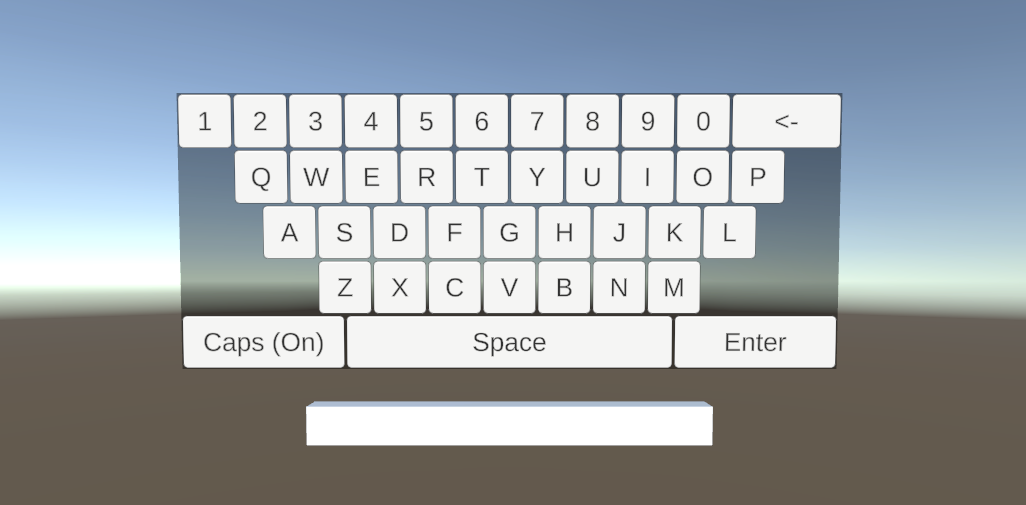
\includegraphics[width=\textwidth]{images/keyboard.png}
  \caption{Custom Keyboard}
  \label{fig:custom_keyboard}
\end{figure}

To facilitate text entry without breaking user immersion, a custom virtual keyboard was engineered (Figure~\ref{fig:custom_keyboard}).
Unlike standard system overlays, this input module features a dynamic ``billboard'' behavior, automatically rotating
to face the user's viewport to ensure optimal legibility. Furthermore, the keyboard is integrated into the world-space interaction system,
allowing users to reposition it freely within their personal reach zone. The software logic supports full alphanumeric input,
including toggles for casing (upper/lower case).

\section{Undo and Redo Actions}

To ensure user experience fluidity and error recovery, \textit{SceneEditorVR}
implements a command-based history system. This is achieved through the \textbf{Command Design Pattern},
which encapsulates every user interaction as a discrete object.

\subsection{The UserAction Interface}
All reversible operations inherit from a primary abstract class, \texttt{UserAction}.
This architecture utilizes polymorphism to allow the system to treat different operations (e.g., transformations, spawning, or selection)
through a unified interface.

\subsection{State Management via Dual Stacks}
The system manages the history using two Last-In-First-Out (LIFO) stacks managed by the \texttt{ActionsManager}:

\begin{itemize}
  \item \textbf{Undo Stack:} Stores executed actions. When a new action is performed, its \texttt{Do()} method is called
        and it is pushed onto this stack.
  \item \textbf{Redo Stack:} Stores actions that have been reversed. If the user performs a new action,
        this stack is cleared to maintain a linear timeline.
\end{itemize}

The implemented actions include spatial transformations (\textit{Move, Rotate, Scale}), object lifecycle management (\textit{Spawn, Delete}),
and selection state changes (\textit{Select, Unselect}).
This modular approach ensures that the system is easily extensible for future features.

\section{Rotation Mechanics Implementation}

The rotation workflow is divided into two main stages:

\subsection{Initialization and Reference Mapping}
Upon interacting with the gizmo, the system captures the initial position and rotation of all selected objects.
If multiple objects are selected, it calculates a shared pivot point.
This ensures that the entire group rotates cohesively as a single unit around a common center of mass.

\subsection{Mathematical Projection and Continuous Update}
Since VR controllers move freely in 3D space, the system must translate this movement into a constrained rotational value.
The script utilizes \texttt{Vector3.ProjectOnPlane}
to mathematically project the controller's 3D movement onto a 2D plane perpendicular to the active rotation axis.
The exact angle is then calculated and applied to the objects. To maintain immersion,
the system concurrently communicates with the \texttt{RotationVisualizerManager} to render a dynamic visual guide
that updates in real-time.

\section{Dual-Camera Rendering Architecture}

To ensure the control panel remains visible and never clips through 3D objects, a dual-camera system was implemented:

\begin{itemize}
  \item \textbf{World Camera} : Renders the environment and all interactive actors.
  \item \textbf{UI Overlay Camera} : Renders only the controllers and the control panel.
\end{itemize}

By assigning the UI Camera a higher depth priority, the control panel is forced to render on top of all world geometry.
This ensures the user never ``loses'' the interface inside walls or large assets.

\section{Asset Management Using Addressables}

To efficiently manage the diverse library of predefined 3D models—categorized into Western, Medieval, Vegetation,
and Primitive Objects—the Unity Addressables System was integrated into the project's architecture.
Traditional asset referencing in Unity requires objects to be loaded into memory synchronously when the scene initializes.
This approach scales poorly as the asset library grows and creates significant performance bottlenecks.
Given the strict memory limitations and processing constraints of standalone VR hardware like the Meta Quest 2,
optimizing the application's memory footprint and load times is critical. Utilizing Addressables establishes a
robust and scalable foundation. While the current prototype relies on locally stored predefined assets, this architecture natively supports
remote content delivery. This design choice paves the way for future iterations where users could seamlessly download
additional themed asset packs from an external server without needing to update the base application.

\chapter{EXPERT EVALUATION}
To assess the usability, efficiency, and overall user experience of \textit{SceneEditorVR}, an expert evaluation study was conducted.
The study was designed to observe how users interact with the spatial interface and to gather qualitative and quantitative feedback regarding
the system's effectiveness.

\section{Experimental Procedure}
Upon arrival, participants were welcomed and briefed on the purpose of the study.
They were provided with information detailing the research objectives and asked to sign a consent form.
Following this, a questionnaire was administered to gather demographic data and assess their prior experience.

\subsection{Participant Information Questionnaire}

The Participant Information Questionnaire was designed to gather essential demographic information
and establish a baseline of the participants' prior technical background. 
Specifically, it collects basic demographic details, including age, gender, dominant hand, and 
whether the participant requires visual correction (glasses) during the VR session. 
To gauge prior exposure to immersive technologies, 
the questionnaire queries participants on their years of experience with VR, their frequency of VR usage, 
their self-reported susceptibility to simulator sickness, and the specific VR headsets they have previously operated. 
Furthermore, the questionnaire evaluates their experience with 3D design and development tools, 
asking them to list any 3D creation software they have used (e.g., Blender, Unity, Unreal Engine), 
rate their proficiency on a 5-point scale, and specify whether they have prior experience with immersive, inside-VR scene editors.
This background data is essential for contextualizing the subsequent evaluation results, as participants' 
familiarity with VR interaction patterns and 3D workflows may influence their performance and adaptation to the system. 
The complete format of this questionnaire is provided in Appendix \ref{appendix:questionnaires}.

\section{Familiarization with the Hardware}
Participants were equipped with a Meta Quest 2 headset and given a brief explanation of the physical boundaries
(room-scale setup) and the basic controller layout to ensure they felt comfortable and safe before entering the virtual environment. A recording of the user's view was initiated to gather information about their experience.

\section{Guided Tutorial Phase}
To familiarize users with the \textit{SceneEditorVR} interaction paradigms, the evaluation began with a guided tutorial phase.
During this stage, participants were asked to complete a series of specific, progressively complex tasks, categorized by the core interactions required.
These tasks were structured into the following categories:

\subsection{Scene Initialization and File Operations}
Participants began by setting up a workspace:
\begin{itemize}
  \item Go to create scene screen
  \item Use the keyboard to give the scene a name (move the keyboard around)
  \item Create scene
\end{itemize}

\subsection{Locomotion and Navigation}
These tasks assessed the user's ability to navigate within the virtual environment:
\begin{itemize}
  \item Rotate around
  \item Move around (vertically and horizontally)
\end{itemize}

\subsection{Control Panel and UI Navigation}
Users practiced summoning and interacting with the central system menus:
\begin{itemize}
  \item Call control panel to user
  \item Inspect content tab in the UI
  \item Inspect scene tab in the UI
  \item Inspect help tab in the UI
\end{itemize}

\subsection{Basic Asset Manipulation}
This phase covered the foundational interactions for selecting, transforming, and editing individual objects:
\begin{itemize}
  \item Drag and drop asset to the scene (move and rotate while dragging)
  \item Deselect asset
  \item Select asset
  \item Move asset
  \item Change transform options using the radial menu
  \item Rotate asset
  \item Scale asset
  \item Open actions radial menu and cancel
  \item Duplicate item and then move new one
  \item Delete duplicated item
  \item Delete original item
  \item Undo
  \item Redo
\end{itemize}

\subsection{Advanced Selection and Multi-Object Manipulation}
Participants performed complex operations involving simultaneous control over multiple objects:
\begin{itemize}
  \item Place four objects in the scene
  \item Multi select all objects
  \item Move multiple objects
  \item Scale multiple objects
  \item Rotate multiple objects
\end{itemize}

\subsection{Snapping and Precision Controls}
These tasks tested the precision positioning constraints and snapping adjustments:
\begin{itemize}
  \item Control snapping amount
  \item Turn off snapping
  \item Move without snap
  \item Scale without snap
  \item Rotate without snap
  \item Save Scene
  \item Export Scene
  \item Menu
  \item Load created scene
\end{itemize}

This phase ensured that all users reached a baseline proficiency with the system's mechanics before moving on to independent creation.

\section{Creation Process}

\subsection{Structured Creation}
In this section, participants were instructed to build a specific layout: a medieval room featuring a central table surrounded by four chairs.
A timer was used to measure completion speed for this task.

\subsection{Free Creation}
In this section, participants were tasked with freely decorating the room they created in the previous section,
using any available assets they chose. During this phase, the recording was used to track errors, undo actions, and deletions.

\section{Questionnaires}
Immediately after concluding the VR session, participants were asked to complete a series of standardized and custom
questionnaires to provide quantitative data on their experience.

\subsection{VRSUQ}
To evaluate the system's usability, the Virtual Reality System Usability Questionnaire (VRSUQ) was administered~\cite{KimRhiu2024VRSUQ}.
This tool is specifically tailored to assess the ease of use, interface intuitiveness,
and overall user satisfaction within immersive spatial computing environments.

The format of this questionnaire is provided in Appendix \ref{appendix:questionnaires}.


\subsection{UEQ-S}
The short version of the User Experience Questionnaire (UEQ-S)~\cite{Schrepp2017UEQS} was utilized to measure
both the pragmatic (efficiency, perspicuity, dependability) and hedonic (stimulation, novelty) qualities
of the software. This provided a quick but comprehensive overview of the users' subjective impressions.

The format of this questionnaire is provided in Appendix \ref{appendix:questionnaires}.


\subsection{Custom Questions}
In addition to the standardized forms, a set of custom questions was designed specifically for this study.
These questions targeted unique features of \textit{SceneEditorVR}, such as the perceived accuracy of the spatial rotation visualizer,
and the comfort of the selected locomotion methods.

The format of this questionnaire is provided in Appendix \ref{appendix:questionnaires}.


\section{Interviews}
The final phase of the evaluation consisted of a semi-structured interview, allowing participants to elaborate on their
questionnaire responses and provide deeper qualitative insights.

\subsection{Open Ended Questions}
The semi-structured interview concluded with the following open-ended questions:

\begin{enumerate}
  \item How was the experience compared to other editors?
  \item What features would make the application better?
  \item What were some positives of the application?
  \item What were some negatives of the application?
\end{enumerate}

\chapter{ANALYSIS AND RESULTS}

% To be completed: Add experimental data and analysis.

\chapter{CONCLUSION}

% To be completed: Add conclusion.

\backmatter

% abbreviations table
\abbreviations
\begin{center}
  \renewcommand{\arraystretch}{1.5}
  \begin{longtable}{| l | @{\qquad} l |}
    \hline
    VR      & Virtual Reality                       \\
    \hline
    3D      & Three Dimensional                     \\
    \hline
    2D      & Two Dimensional                       \\
    \hline
    6DoF    & Six Degrees of Freedom                \\
    \hline
    UGC     & User Generated Content                \\
    \hline
    UI      & User Interface                        \\
    \hline
    WIMP    & Windows Icons Menus Pointers          \\
    \hline
    XR      & Extended Reality                      \\
    \hline
    UX      & User Experience                       \\
    \hline
    AEC     & Architecture Engineering Construction \\
    \hline
    WYSIWYG & What You See Is What You Get          \\
    \hline
  \end{longtable}
\end{center}

\begin{appendix}
  \appendixstartedtrue

  % add appendix line to ToC
  \phantomsection
  \addcontentsline{toc}{chapter}{APPENDICES}

  \chapter{QUESTIONNAIRES}
  \label{appendix:questionnaires}

  \section{Participant Information Questionnaire}
  \begin{enumerate}
    \item \textbf{Age}
          \textit{(Number Input)}

    \item \textbf{Gender}
          \begin{itemize}
            \item Male
            \item Female
            \item Prefer not to answer
          \end{itemize}

    \item \textbf{Which is your dominant hand?}
          \begin{itemize}
            \item Right
            \item Left
            \item Both
          \end{itemize}

    \item \textbf{Do you wear glasses? Will you be wearing them during the VR experiment?}
          \begin{itemize}
            \item No I don't wear glasses
            \item Yes I wear glasses and I will be wearing them during the experiment
            \item Yes I wear glasses but I will not be wearing them during the experiment
          \end{itemize}

    \item \textbf{Years of experience with VR}
          \begin{itemize}
            \item Less than a year
            \item 1-3 years
            \item More than 3 years
          \end{itemize}

    \item \textbf{How often are you in VR?}
          \begin{itemize}
            \item 0 times per month
            \item 1-3 times per month
            \item 1-2 times per week
            \item 3-5 times per week
            \item Every day
          \end{itemize}

    \item \begin{minipage}[t]{\linewidth}
            \textbf{How easily do you get motion sickness in VR?}
            \begin{center}
              \small
              \renewcommand{\arraystretch}{1.5}
              \begin{tabular}{ccccccccc}
                            & 1          & 2          & 3          & 4          & 5          &            \\
                Very easily & $\bigcirc$ & $\bigcirc$ & $\bigcirc$ & $\bigcirc$ & $\bigcirc$ & I get none
              \end{tabular}
            \end{center}
          \end{minipage}

    \item \textbf{Which VR devices have you used?}
          \textit{(Text Input)}

    \item \textbf{What tools have you used for 3D scene creation (Blender, Unity, Unreal Engine etc.)?}
          \textit{(Text Input)}

    \item \begin{minipage}[t]{\linewidth}
            \textbf{What is your experience level in the tools you mentioned in the last question?}
            \begin{center}
              \small
              \renewcommand{\arraystretch}{1.5}
              \begin{tabular}{ccccccccc}
                         & 1          & 2          & 3          & 4          & 5          &            \\
                Beginner & $\bigcirc$ & $\bigcirc$ & $\bigcirc$ & $\bigcirc$ & $\bigcirc$ & Proficient
              \end{tabular}
            \end{center}
          \end{minipage}

    \item \textbf{Have you used a tool for scene creation inside VR? If yes, which ones have you used?}
          \textit{(Text Input)}

  \end{enumerate}

  \section{VRSUQ}
  \begin{enumerate}
    \item \begin{minipage}[t]{\linewidth}
            \textbf{The system responded well to my manipulations as expected with no delays.}
            \begin{center}
              \small
              \renewcommand{\arraystretch}{1.5}
              \begin{tabular}{ccccccccc}
                                  & 1          & 2          & 3          & 4          & 5          & 6          & 7          &                \\
                Strongly Disagree & $\bigcirc$ & $\bigcirc$ & $\bigcirc$ & $\bigcirc$ & $\bigcirc$ & $\bigcirc$ & $\bigcirc$ & Strongly Agree
              \end{tabular}
            \end{center}
          \end{minipage}

    \item \begin{minipage}[t]{\linewidth}
            \textbf{I think the virtual reality system provides clear feedback on my manipulations.}
            \begin{center}
              \small
              \renewcommand{\arraystretch}{1.5}
              \begin{tabular}{ccccccccc}
                                  & 1          & 2          & 3          & 4          & 5          & 6          & 7          &                \\
                Strongly Disagree & $\bigcirc$ & $\bigcirc$ & $\bigcirc$ & $\bigcirc$ & $\bigcirc$ & $\bigcirc$ & $\bigcirc$ & Strongly Agree
              \end{tabular}
            \end{center}
          \end{minipage}


    \item \begin{minipage}[t]{\linewidth}
            \textbf{(−)I kept making errors/mistakes while using the virtual reality system.}
            \begin{center}
              \small
              \renewcommand{\arraystretch}{1.5}
              \begin{tabular}{ccccccccc}
                                  & 1          & 2          & 3          & 4          & 5          & 6          & 7          &                \\
                Strongly Disagree & $\bigcirc$ & $\bigcirc$ & $\bigcirc$ & $\bigcirc$ & $\bigcirc$ & $\bigcirc$ & $\bigcirc$ & Strongly Agree
              \end{tabular}
            \end{center}
          \end{minipage}


    \item \begin{minipage}[t]{\linewidth}
            \textbf{I could clearly understand the information presented within the virtual environment.}
            \begin{center}
              \small
              \renewcommand{\arraystretch}{1.5}
              \begin{tabular}{ccccccccc}
                                  & 1          & 2          & 3          & 4          & 5          & 6          & 7          &                \\
                Strongly Disagree & $\bigcirc$ & $\bigcirc$ & $\bigcirc$ & $\bigcirc$ & $\bigcirc$ & $\bigcirc$ & $\bigcirc$ & Strongly Agree
              \end{tabular}
            \end{center}
          \end{minipage}


    \item \begin{minipage}[t]{\linewidth}
            \textbf{I think this system is user-friendly, straightforward to learn, and designed in such a way that most people will find it easy to adapt to.}
            \begin{center}
              \small
              \renewcommand{\arraystretch}{1.5}
              \begin{tabular}{ccccccccc}
                                  & 1          & 2          & 3          & 4          & 5          & 6          & 7          &                \\
                Strongly Disagree & $\bigcirc$ & $\bigcirc$ & $\bigcirc$ & $\bigcirc$ & $\bigcirc$ & $\bigcirc$ & $\bigcirc$ & Strongly Agree
              \end{tabular}
            \end{center}
          \end{minipage}


    \item \begin{minipage}[t]{\linewidth}
            \textbf{I think it is easy to correct errors made while using the virtual reality system.}
            \begin{center}
              \small
              \renewcommand{\arraystretch}{1.5}
              \begin{tabular}{ccccccccc}
                                  & 1          & 2          & 3          & 4          & 5          & 6          & 7          &                \\
                Strongly Disagree & $\bigcirc$ & $\bigcirc$ & $\bigcirc$ & $\bigcirc$ & $\bigcirc$ & $\bigcirc$ & $\bigcirc$ & Strongly Agree
              \end{tabular}
            \end{center}
          \end{minipage}


    \item \begin{minipage}[t]{\linewidth}
            \textbf{I enjoyed the virtual reality experience.}
            \begin{center}
              \small
              \renewcommand{\arraystretch}{1.5}
              \begin{tabular}{ccccccccc}
                                  & 1          & 2          & 3          & 4          & 5          & 6          & 7          &                \\
                Strongly Disagree & $\bigcirc$ & $\bigcirc$ & $\bigcirc$ & $\bigcirc$ & $\bigcirc$ & $\bigcirc$ & $\bigcirc$ & Strongly Agree
              \end{tabular}
            \end{center}
          \end{minipage}


    \item \begin{minipage}[t]{\linewidth}
            \textbf{(−) I felt dizzy, motion sickness, or a headache while experiencing virtual reality.}
            \begin{center}
              \small
              \renewcommand{\arraystretch}{1.5}
              \begin{tabular}{ccccccccc}
                                  & 1          & 2          & 3          & 4          & 5          & 6          & 7          &                \\
                Strongly Disagree & $\bigcirc$ & $\bigcirc$ & $\bigcirc$ & $\bigcirc$ & $\bigcirc$ & $\bigcirc$ & $\bigcirc$ & Strongly Agree
              \end{tabular}
            \end{center}
          \end{minipage}


    \item \begin{minipage}[t]{\linewidth}
            \textbf{(−) While experiencing virtual reality, I felt mental burdens such as tension, frustration, and time pressure.}
            \begin{center}
              \small
              \renewcommand{\arraystretch}{1.5}
              \begin{tabular}{ccccccccc}
                                  & 1          & 2          & 3          & 4          & 5          & 6          & 7          &                \\
                Strongly Disagree & $\bigcirc$ & $\bigcirc$ & $\bigcirc$ & $\bigcirc$ & $\bigcirc$ & $\bigcirc$ & $\bigcirc$ & Strongly Agree
              \end{tabular}
            \end{center}
          \end{minipage}
  \end{enumerate}

  \section{UEQ-S}
  \begin{enumerate}
    \item \begin{minipage}[t]{\linewidth}
            \textbf{obstructive vs. supportive}
            \begin{center}
              \small
              \renewcommand{\arraystretch}{1.5}
              \begin{tabular}{ccccccccc}
                            & 1          & 2          & 3          & 4          & 5          & 6          & 7          &            \\
                obstructive & $\bigcirc$ & $\bigcirc$ & $\bigcirc$ & $\bigcirc$ & $\bigcirc$ & $\bigcirc$ & $\bigcirc$ & supportive
              \end{tabular}
            \end{center}
          \end{minipage}


    \item \begin{minipage}[t]{\linewidth}
            \textbf{complicated vs. easy}
            \begin{center}
              \small
              \renewcommand{\arraystretch}{1.5}
              \begin{tabular}{ccccccccc}
                            & 1          & 2          & 3          & 4          & 5          & 6          & 7          &      \\
                complicated & $\bigcirc$ & $\bigcirc$ & $\bigcirc$ & $\bigcirc$ & $\bigcirc$ & $\bigcirc$ & $\bigcirc$ & easy
              \end{tabular}
            \end{center}
          \end{minipage}


    \item \begin{minipage}[t]{\linewidth}
            \textbf{inefficient vs. efficient}
            \begin{center}
              \small
              \renewcommand{\arraystretch}{1.5}
              \begin{tabular}{ccccccccc}
                            & 1          & 2          & 3          & 4          & 5          & 6          & 7          &           \\
                inefficient & $\bigcirc$ & $\bigcirc$ & $\bigcirc$ & $\bigcirc$ & $\bigcirc$ & $\bigcirc$ & $\bigcirc$ & efficient
              \end{tabular}
            \end{center}
          \end{minipage}


    \item \begin{minipage}[t]{\linewidth}
            \textbf{clear vs. confusing}
            \begin{center}
              \small
              \renewcommand{\arraystretch}{1.5}
              \begin{tabular}{ccccccccc}
                      & 1          & 2          & 3          & 4          & 5          & 6          & 7          &           \\
                clear & $\bigcirc$ & $\bigcirc$ & $\bigcirc$ & $\bigcirc$ & $\bigcirc$ & $\bigcirc$ & $\bigcirc$ & confusing
              \end{tabular}
            \end{center}
          \end{minipage}


    \item \begin{minipage}[t]{\linewidth}
            \textbf{boring  vs. exciting}
            \begin{center}
              \small
              \renewcommand{\arraystretch}{1.5}
              \begin{tabular}{ccccccccc}
                       & 1          & 2          & 3          & 4          & 5          & 6          & 7          &          \\
                boring & $\bigcirc$ & $\bigcirc$ & $\bigcirc$ & $\bigcirc$ & $\bigcirc$ & $\bigcirc$ & $\bigcirc$ & exciting
              \end{tabular}
            \end{center}
          \end{minipage}

    \item \begin{minipage}[t]{\linewidth}
            \textbf{not interesting vs. interesting}
            \begin{center}
              \small
              \renewcommand{\arraystretch}{1.5}
              \begin{tabular}{ccccccccc}
                                & 1          & 2          & 3          & 4          & 5          & 6          & 7          &             \\
                not interesting & $\bigcirc$ & $\bigcirc$ & $\bigcirc$ & $\bigcirc$ & $\bigcirc$ & $\bigcirc$ & $\bigcirc$ & interesting
              \end{tabular}
            \end{center}
          \end{minipage}


    \item \begin{minipage}[t]{\linewidth}
            \textbf{conventional vs. inventive}
            \begin{center}
              \small
              \renewcommand{\arraystretch}{1.5}
              \begin{tabular}{ccccccccc}
                             & 1          & 2          & 3          & 4          & 5          & 6          & 7          &           \\
                conventional & $\bigcirc$ & $\bigcirc$ & $\bigcirc$ & $\bigcirc$ & $\bigcirc$ & $\bigcirc$ & $\bigcirc$ & inventive
              \end{tabular}
            \end{center}
          \end{minipage}


    \item \begin{minipage}[t]{\linewidth}
            \textbf{usual vs. leading-edge}
            \begin{center}
              \small
              \renewcommand{\arraystretch}{1.5}
              \begin{tabular}{ccccccccc}
                      & 1          & 2          & 3          & 4          & 5          & 6          & 7          &              \\
                usual & $\bigcirc$ & $\bigcirc$ & $\bigcirc$ & $\bigcirc$ & $\bigcirc$ & $\bigcirc$ & $\bigcirc$ & leading-edge
              \end{tabular}
            \end{center}
          \end{minipage}
  \end{enumerate}

  \section{Custom Questions}
  \begin{enumerate}
    \item \begin{minipage}[t]{\linewidth}
            \textbf{How easy was it to transform the assets in the scene?}
            \begin{center}
              \small
              \renewcommand{\arraystretch}{1.5}
              \begin{tabular}{ccccccc}
                               & 1          & 2          & 3          & 4          & 5          &           \\
                Very difficult & $\bigcirc$ & $\bigcirc$ & $\bigcirc$ & $\bigcirc$ & $\bigcirc$ & Very easy
              \end{tabular}
            \end{center}
          \end{minipage}

    \item \begin{minipage}[t]{\linewidth}
            \textbf{How intuitive was the rotation of the objects?}
            \begin{center}
              \small
              \renewcommand{\arraystretch}{1.5}
              \begin{tabular}{ccccccc}
                            & 1          & 2          & 3          & 4          & 5          &                \\
                Unintuitive & $\bigcirc$ & $\bigcirc$ & $\bigcirc$ & $\bigcirc$ & $\bigcirc$ & Very intuitive
              \end{tabular}
            \end{center}
          \end{minipage}

    \item \begin{minipage}[t]{\linewidth}
            \textbf{Was the central UI panel during the scene creation intrusive?}
            \begin{center}
              \small
              \renewcommand{\arraystretch}{1.5}
              \begin{tabular}{ccccccc}
                               & 1          & 2          & 3          & 4          & 5          &               \\
                Very Intrusive & $\bigcirc$ & $\bigcirc$ & $\bigcirc$ & $\bigcirc$ & $\bigcirc$ & Not Intrusive
              \end{tabular}
            \end{center}
          \end{minipage}

    \item \begin{minipage}[t]{\linewidth}
            \textbf{How helpful was the snapping system?}
            \begin{center}
              \small
              \renewcommand{\arraystretch}{1.5}
              \begin{tabular}{ccccccc}
                            & 1          & 2          & 3          & 4          & 5          &              \\
                Not helpful & $\bigcirc$ & $\bigcirc$ & $\bigcirc$ & $\bigcirc$ & $\bigcirc$ & Very helpful
              \end{tabular}
            \end{center}
          \end{minipage}

    \item \begin{minipage}[t]{\linewidth}
            \textbf{How easy was it to navigate around the scene?}
            \begin{center}
              \small
              \renewcommand{\arraystretch}{1.5}
              \begin{tabular}{ccccccc}
                          & 1          & 2          & 3          & 4          & 5          &           \\
                Very hard & $\bigcirc$ & $\bigcirc$ & $\bigcirc$ & $\bigcirc$ & $\bigcirc$ & Very easy
              \end{tabular}
            \end{center}
          \end{minipage}

    \item \begin{minipage}[t]{\linewidth}
            \textbf{Would you prefer to make virtual reality scenes with this tool, rather than a traditional scene editor?}
            \begin{center}
              \small
              \renewcommand{\arraystretch}{1.5}
              \begin{tabular}{ccccccc}
                           & 1          & 2          & 3          & 4          & 5          &             \\
                Not likely & $\bigcirc$ & $\bigcirc$ & $\bigcirc$ & $\bigcirc$ & $\bigcirc$ & Most likely
              \end{tabular}
            \end{center}
          \end{minipage}
  \end{enumerate}

\end{appendix}

% manually include the bibliography
\bibliographystyle{plain}
{\footnotesize \bibliography{references}}

\addcontentsline{toc}{chapter}{REFERENCES}

\end{document}